\input{"preamble.tex"}

\addbibresource{Complex\_Analysis\_Problems.bib}

\let\Begin\begin
\let\End\end
\newcommand\wrapenv[1]{#1}

\makeatletter
\def\ScaleWidthIfNeeded{%
 \ifdim\Gin@nat@width>\linewidth
    \linewidth
  \else
    \Gin@nat@width
  \fi
}
\def\ScaleHeightIfNeeded{%
  \ifdim\Gin@nat@height>0.9\textheight
    0.9\textheight
  \else
    \Gin@nat@width
  \fi
}
\makeatother

\setkeys{Gin}{width=\ScaleWidthIfNeeded,height=\ScaleHeightIfNeeded,keepaspectratio}%

\title{
\textbf{
    Complex Analysis Qualifying Exam Questions
  }
  }







\begin{document}

\date{}
\author{D. Zack Garza}
\maketitle


\newpage

% Note: addsec only in KomaScript
\addsec{Table of Contents}
\tableofcontents
\newpage

\hypertarget{preface}{%
\section{Preface}\label{preface}}

I'd like to thank the following individuals for their contributions to
this document:

\begin{itemize}
\tightlist
\item
  Edward Azoff, for supplying a problem sheet broken out by topic.
\item
  Mentzelos Melistas, for explaining and documenting many solutions to
  these questions.
\item
  Jingzhi Tie, for supplying many additional problems and solutions.
\end{itemize}

\hypertarget{topology-and-functions-of-one-variable-8155a}{%
\section{Topology and Functions of One Variable
(8155a)}\label{topology-and-functions-of-one-variable-8155a}}

\hypertarget{work}{%
\subsection{\texorpdfstring{1
\(\work\)}{1 \textbackslash work}}\label{work}}

Let \(x_0 = a, x_1 = b\), and set
\begin{align*}  
x_n \coloneqq{x_{n-1} + x_{n-2} \over 2} \quad n\geq 2
.\end{align*}

Show that \(\left\{{x_n}\right\}\) is a Cauchy sequence and find its
limit in terms of \(a\) and \(b\).

\hypertarget{work-1}{%
\subsection{\texorpdfstring{2
\(\work\)}{2 \textbackslash work}}\label{work-1}}

Suppose \(f:{\mathbb{R}}\to{\mathbb{R}}\) is continuous and
\(\lim_{x\to \pm \infty} f(x) = 0\). Prove that \(f\) is uniformly
continuous.

\hypertarget{work-2}{%
\subsection{\texorpdfstring{3
\(\work\)}{3 \textbackslash work}}\label{work-2}}

Give an example of a function \(f:{\mathbb{R}}\to {\mathbb{R}}\) that is
everywhere differentiable but \(f'\) is not continuous at 0.

\hypertarget{work-3}{%
\subsection{\texorpdfstring{4
\(\work\)}{4 \textbackslash work}}\label{work-3}}

Suppose \(\left\{{g_n}\right\}\) is a uniformly convergent sequence of
functions from \({\mathbb{R}}\) to \({\mathbb{R}}\) and
\(f:{\mathbb{R}}\to {\mathbb{R}}\) is uniformly continuous. Prove that
the sequence \(\left\{{f\circ g_n}\right\}\) is uniformly convergent.

\hypertarget{work-4}{%
\subsection{\texorpdfstring{5
\(\work\)}{5 \textbackslash work}}\label{work-4}}

Let \(f\) be differentiable on \([a, b]\). Say that \(f\) is
\emph{uniformly differentiable} iff

\begin{align*}  
\forall \varepsilon > 0,\, \exists \delta > 0 \text{ such that } \quad {\left\lvert {x-y} \right\rvert} < \delta \implies {\left\lvert { {f(x) - f(y) \over x-y}  - f'(y)} \right\rvert}  < \varepsilon
.\end{align*}

Prove that \(f\) is uniformly differentiable on \([a, b] \iff f'\) is
continuous on \([a, b]\).

\hypertarget{work-5}{%
\subsection{\texorpdfstring{6
\(\work\)}{6 \textbackslash work}}\label{work-5}}

Suppose \(A, B \subseteq {\mathbb{R}}^n\) are disjoint and compact.
Prove that there exist \(a\in A, b\in B\) such that
\begin{align*}  
{\left\lVert {a - b} \right\rVert} = \inf\left\{{{\left\lVert {x-y} \right\rVert} {~\mathrel{\Big|}~}x\in A,\, y\in B}\right\}
.\end{align*}

\hypertarget{work-6}{%
\subsection{\texorpdfstring{7
\(\work\)}{7 \textbackslash work}}\label{work-6}}

Suppose \(A, B\subseteq {\mathbb{R}}^n\) are connected and not disjoint.
Prove that \(A\cup B\) is also connected.

\hypertarget{work-7}{%
\subsection{\texorpdfstring{8
\(\work\)}{8 \textbackslash work}}\label{work-7}}

Suppose \(\left\{{f_n}\right\}_{n\in {\mathbb{N}}}\) is a sequence of
continuous functions \(f_n: [0, 1]\to {\mathbb{R}}\) such that
\begin{align*}  
f_n(x) \geq f_{n+1}(x) \geq 0 \quad \forall n\in {\mathbb{N}},\, \forall x\in [0, 1]
.\end{align*}
Prove that if \(\left\{{f_n}\right\}\) converges pointwise to \(0\) on
\([0, 1]\) then it converges to \(0\) uniformly on \([0, 1]\).

\hypertarget{work-8}{%
\subsection{\texorpdfstring{9
\(\work\)}{9 \textbackslash work}}\label{work-8}}

Show that if \(E\subset [0, 1]\) is uncountable, then there is some
\(t\in {\mathbb{R}}\) such that \(E\cap(-\infty ,t)\) and
\(E\cap(t, \infty)\) are also uncountable.

\hypertarget{several-variables-8155h}{%
\section{Several Variables (8155h)}\label{several-variables-8155h}}

\hypertarget{work-9}{%
\subsection{\texorpdfstring{1
\(\work\)}{1 \textbackslash work}}\label{work-9}}

Is the following function continuous, differentiable, continuously
differentiable?
\begin{align*}  
f: {\mathbb{R}}^2 &\to {\mathbb{R}}\\
f(x, y) &= 
\begin{cases}
{xy \over \sqrt{x^2 + y^2}} & (x, y) \neq (0, 0) \\
0 & \text{else}.
\end{cases}
\end{align*}

\hypertarget{work-10}{%
\subsection{\texorpdfstring{2
\(\work\)}{2 \textbackslash work}}\label{work-10}}

\hypertarget{a-work}{%
\subsubsection{\texorpdfstring{a
\(\work\)}{a \textbackslash work}}\label{a-work}}

Complete this definition: ``\(f: {\mathbb{R}}^n\to {\mathbb{R}}^m\) is
real-differentiable a point \(p\in {\mathbb{R}}^n\) iff there exists a
linear transformation\ldots{}''

\hypertarget{b-work}{%
\subsubsection{\texorpdfstring{b
\(\work\)}{b \textbackslash work}}\label{b-work}}

Give an example of a function \(f:{\mathbb{R}}^2\to {\mathbb{R}}\) whose
first-order partial derivatives exist everywhere but \(f\) is not
differentiable at \((0, 0)\).

\hypertarget{c-work}{%
\subsubsection{\texorpdfstring{c
\(\work\)}{c \textbackslash work}}\label{c-work}}

Give an example of a function \(f: {\mathbb{R}}^2 \to {\mathbb{R}}\)
which is real-differentiable everywhere but nowhere
complex-differentiable.

\hypertarget{work-11}{%
\subsection{\texorpdfstring{3
\(\work\)}{3 \textbackslash work}}\label{work-11}}

Let \(f:{\mathbb{R}}^2\to {\mathbb{R}}\).

\hypertarget{a-work-1}{%
\subsubsection{\texorpdfstring{a
\(\work\)}{a \textbackslash work}}\label{a-work-1}}

Define in terms of linear transformations what it means for \(f\) to be
differentiable at a point \((a, b) \in {\mathbb{R}}^2\).

\hypertarget{b-work-1}{%
\subsubsection{\texorpdfstring{b
\(\work\)}{b \textbackslash work}}\label{b-work-1}}

State a version of the inverse function theorem in this setting.

\hypertarget{c-work-1}{%
\subsubsection{\texorpdfstring{c
\(\work\)}{c \textbackslash work}}\label{c-work-1}}

Identify \({\mathbb{R}}^2\) with \({\mathbb{C}}\) and give a necessary
and sufficient condition for a real-differentiable function at
\((a, b)\) to be complex differentiable at the point \(a+ib\).

\hypertarget{work-12}{%
\subsection{\texorpdfstring{4
\(\work\)}{4 \textbackslash work}}\label{work-12}}

Let \(f = u+iv\) be complex-differentiable with continuous partial
derivatives at a point \(z = re^{i\theta}\) with \(r\neq 0\). Show that
\begin{align*}  
{\frac{\partial u}{\partial r}\,} = {1\over r}{\frac{\partial v}{\partial \theta}\,} \qquad {\frac{\partial v}{\partial r}\,} = -{1\over r}{\frac{\partial u}{\partial \theta}\,}
.\end{align*}

\hypertarget{work-13}{%
\subsection{\texorpdfstring{5
\(\work\)}{5 \textbackslash work}}\label{work-13}}

Let \(P = (1, 3) \in {\mathbb{R}}^2\) and define
\begin{align*}  
f(s, t) \coloneqq ps^3 -6st + t^2
.\end{align*}

\hypertarget{a-work-2}{%
\subsubsection{\texorpdfstring{a
\(\work\)}{a \textbackslash work}}\label{a-work-2}}

State the conclusion of the implicit function theorem concerning
\(f(s, t) = 0\) when \(f\) is considered a function
\({\mathbb{R}}^2\to{\mathbb{R}}\).

\hypertarget{b-work-2}{%
\subsubsection{\texorpdfstring{b
\(\work\)}{b \textbackslash work}}\label{b-work-2}}

State the above conclusion when \(f\) is considered a function
\({\mathbb{C}}^2\to {\mathbb{C}}\).

\hypertarget{c-work-2}{%
\subsubsection{\texorpdfstring{c
\(\work\)}{c \textbackslash work}}\label{c-work-2}}

Use the implicit function theorem for a function
\({\mathbb{R}}\times{\mathbb{R}}^2 \to {\mathbb{R}}^2\) to prove (b).

\begin{quote}
There are various approaches: using the definition of the complex
derivative, the Cauchy-Riemann equations, considering total derivatives,
etc.
\end{quote}

\hypertarget{work-14}{%
\subsection{\texorpdfstring{6
\(\work\)}{6 \textbackslash work}}\label{work-14}}

Let \(F:{\mathbb{R}}^2\to {\mathbb{R}}\) be continuously differentiable
with \(F(0, 0) = 0\) and
\({\left\lVert {\nabla F(0, 0)} \right\rVert} < 1\).

Prove that there is some real number \(r> 0\) such that
\({\left\lvert {F(x, y)} \right\rvert} < r\) whenever
\({\left\lVert {(x, y)} \right\rVert} < r\).

\hypertarget{work-15}{%
\subsection{\texorpdfstring{7
\(\work\)}{7 \textbackslash work}}\label{work-15}}

State the most general version of the implicit function theorem for real
functions and outline how it can be proved using the inverse function
theorem.

\hypertarget{several-variables-extra-questions}{%
\section{Several Variables: Extra
Questions}\label{several-variables-extra-questions}}

\hypertarget{section}{%
\subsection{?}\label{section}}

Let \(f=u+iv\) be differentiable (i.e.~\(f'(z)\) exists) with continuous
partial derivatives at a point \(z=re^{i\theta}\), \(r\not= 0\).

Show that
\begin{align*}
\frac{\partial u}{\partial r}=\frac{1}{r}\frac{\partial v}{\partial \theta},\quad
\frac{\partial v}{\partial r}=-\frac{1}{r}\frac{\partial u}{\partial \theta}
.\end{align*}

\hypertarget{section-1}{%
\subsection{?}\label{section-1}}

Give an example of a

Show that \(f(z) = z^2\) is uniformly continuous in any open disk
\(|z| < R\), where \(R>0\) is fixed, but it is not uniformly continuous
on \(\mathbb C\).

\hypertarget{section-2}{%
\subsubsection{1}\label{section-2}}

Show that the function \(u=u(x,y)\) given by
\begin{align*}
u(x,y)=\frac{e^{ny}-e^{-ny}}{2n^2}\sin nx\quad \text{for}\ n\in {\mathbf N}
\end{align*}
is the solution on \(D=\{(x,y)\ | x^2+y^2<1\}\) of the Cauchy problem
for the Laplace equation
\begin{align*}\frac{\partial ^2u}{\partial x^2}+\frac{\partial ^2u}{\partial y^2}=0,\quad
u(x,0)=0,\quad \frac{\partial u}{\partial y}(x,0)=\frac{\sin nx}{n}.\end{align*}

\hypertarget{section-3}{%
\subsubsection{2}\label{section-3}}

Show that there exist points \((x,y)\in D\) such that
\(\displaystyle{\limsup_{n\to\infty} |u(x,y)|=\infty}\).

\hypertarget{conformal-maps-8155c}{%
\section{Conformal Maps (8155c)}\label{conformal-maps-8155c}}

\begin{quote}
Notation: \({\mathbb{D}}\) is the open unit disc, \({\mathbb{H}}\) is
the open upper half-plane.
\end{quote}

\hypertarget{work-16}{%
\subsection{\texorpdfstring{1
\(\work\)}{1 \textbackslash work}}\label{work-16}}

Find a conformal map from \({\mathbb{D}}\) to \({\mathbb{H}}\).

\hypertarget{work-17}{%
\subsection{\texorpdfstring{2
\(\work\)}{2 \textbackslash work}}\label{work-17}}

Find a conformal map from the strip
\(\left\{{z\in {\mathbb{C}}{~\mathrel{\Big|}~}0 < \Im(z) < 1}\right\}\)
to \({\mathbb{H}}\).

\hypertarget{work-18}{%
\subsection{\texorpdfstring{3
\(\work\)}{3 \textbackslash work}}\label{work-18}}

Find a fractional linear transformation \(T\) which maps
\({\mathbb{H}}\) to \({\mathbb{D}}\), and explicitly describe the image
of the first quadrant under \(T\).

\hypertarget{work-19}{%
\subsection{\texorpdfstring{4
\(\work\)}{4 \textbackslash work}}\label{work-19}}

Find a conformal map from
\(\left\{{z\in {\mathbb{C}}{~\mathrel{\Big|}~}{\left\lvert {z-i} \right\rvert} > 1,\, \Re(z) > 0}\right\}\)
to \({\mathbb{H}}\).

\hypertarget{work-20}{%
\subsection{\texorpdfstring{5
\(\work\)}{5 \textbackslash work}}\label{work-20}}

Find a conformal map from
\(\left\{{z\in {\mathbb{C}}{~\mathrel{\Big|}~}{\left\lvert {z} \right\rvert} < 1,\, {\left\lvert {z - {1\over 2}} \right\rvert} > {1\over 2} }\right\}\)
to \({\mathbb{D}}\).

\hypertarget{work-21}{%
\subsection{\texorpdfstring{6
\(\work\)}{6 \textbackslash work}}\label{work-21}}

Find a conformal map from
\(\left\{{{\left\lvert {z-1} \right\rvert} < 2}\right\} \cap\left\{{{\left\lvert {z+1} \right\rvert} < 2}\right\}\)
to \({\mathbb{H}}\).

\hypertarget{work-22}{%
\subsection{\texorpdfstring{7
\(\work\)}{7 \textbackslash work}}\label{work-22}}

Let \(\Omega\) be the region inside the unit circle
\({\left\lvert {z} \right\rvert} = 1\) and outside the circle
\({\left\lvert {z-{1\over 4}} \right\rvert} = {1\over 4}\).

Find an injective conformal map from \(\Omega\) onto some annulus
\(\left\{{r < {\left\lvert {z} \right\rvert} < 1}\right\}\) for gonstant
\(r\).

\hypertarget{work-23}{%
\subsection{\texorpdfstring{8
\(\work\)}{8 \textbackslash work}}\label{work-23}}

Let \(D\) be the region obtained by deleting the real interval
\([0, 1)\) from \({\mathbb{D}}\); find a conformal map from \(D\) to
\({\mathbb{D}}\).

\hypertarget{work-24}{%
\subsection{\texorpdfstring{9
\(\work\)}{9 \textbackslash work}}\label{work-24}}

Find a conformal map from
\({\mathbb{C}}\setminus\left\{{x\in {\mathbb{R}}{~\mathrel{\Big|}~}x\leq 0}\right\}\)
to \({\mathbb{D}}\).

\hypertarget{work-25}{%
\subsection{\texorpdfstring{10
\(\work\)}{10 \textbackslash work}}\label{work-25}}

Find a conformal map from
\({\mathbb{C}}\setminus\left\{{x\in {\mathbb{R}}{~\mathrel{\Big|}~}x\geq 1}\right\}\)
to \({\mathbb{D}}\).

\hypertarget{work-26}{%
\subsection{\texorpdfstring{11
\(\work\)}{11 \textbackslash work}}\label{work-26}}

Find a bijective conformal map from \(G\) to \({\mathbb{H}}\), where
\begin{align*}  
G \coloneqq\left\{{z\in {\mathbb{C}}{~\mathrel{\Big|}~}{\left\lvert {z-1} \right\rvert} < \sqrt 2,\, {\left\lvert {z+1} \right\rvert} < \sqrt 2}\right\} \setminus [0, i)
.\end{align*}

\hypertarget{work-27}{%
\subsection{\texorpdfstring{12
\(\work\)}{12 \textbackslash work}}\label{work-27}}

Prove that TFAE for a Möbius transformation \(T\) given by
\(T(z) = {az + b \over cz + d}\):

\begin{enumerate}
\def\labelenumi{\alph{enumi}.}
\tightlist
\item
  \(T\) maps \({\mathbb{R}}\cup\left\{{\infty}\right\}\) to itself.
\item
  It is possible to choose \(a,b,c,d\) to be real numbers.
\item
  \(\mkern 1.5mu\overline{\mkern-1.5muT(z)\mkern-1.5mu}\mkern 1.5mu = T(\mkern 1.5mu\overline{\mkern-1.5muz\mkern-1.5mu}\mkern 1.5mu)\)
  for every \(z\in {\mathbb{CP}}^1\).
\item
  There exist
  \(\alpha\in {\mathbb{R}}, \beta \in {\mathbb{C}}\setminus {\mathbb{R}}\)
  such that \(T(\alpha) = \alpha\) and
  \(T(\mkern 1.5mu\overline{\mkern-1.5mu\beta\mkern-1.5mu}\mkern 1.5mu) = \mkern 1.5mu\overline{\mkern-1.5muT(\beta)\mkern-1.5mu}\mkern 1.5mu\).
\end{enumerate}

\hypertarget{extra-questions}{%
\section{Extra Questions}\label{extra-questions}}

\hypertarget{section-4}{%
\subsection{12.}\label{section-4}}

Find a conformal map from \(D = \{z :\  |z| < 1,\ |z - 1/2| > 1/2\}\) to
the unit disk \(\Delta=\{z: \ |z|<1\}\).

\hypertarget{integrals-and-cauchys-theorem-8155d}{%
\section{Integrals and Cauchy's Theorem
(8155d)}\label{integrals-and-cauchys-theorem-8155d}}

\begin{quote}
Some interesting problems: 3, 4, 9, 10.
\end{quote}

\hypertarget{work-28}{%
\subsection{\texorpdfstring{1
\(\work\)}{1 \textbackslash work}}\label{work-28}}

Suppose \(f, g: [0, 1] \to {\mathbb{R}}\) where \(f\) is Riemann
integrable and for \(x, y\in [0, 1]\),
\begin{align*}
{\left\lvert {g(x) - g(y)} \right\rvert} \leq {\left\lvert {f(x) - f(y)} \right\rvert}
.\end{align*}

Prove that \(g\) is Riemann integrable.

\hypertarget{work-29}{%
\subsection{\texorpdfstring{2
\(\work\)}{2 \textbackslash work}}\label{work-29}}

State and prove Green's Theorem for rectangles.

Then use it to prove Cauchy's Theory for functions that are analytic in
a rectangle.

\hypertarget{work-30}{%
\subsection{\texorpdfstring{3
\(\work\)}{3 \textbackslash work}}\label{work-30}}

Suppose \(\left\{{f_n}\right\}_{n\in {\mathbb{N}}}\) is a sequence of
analytic functions on
\({\mathbb{D}}\coloneqq\left\{{z\in {\mathbb{C}}{~\mathrel{\Big|}~}{\left\lvert {z} \right\rvert} < 1}\right\}\).

Show that if \(f_n\to g\) for some \(g: {\mathbb{D}}\to {\mathbb{C}}\)
uniformly on every compact \(K\subset {\mathbb{D}}\), then \(g\) is
analytic on \({\mathbb{D}}\).

\hypertarget{work-31}{%
\subsection{\texorpdfstring{4
\(\work\)}{4 \textbackslash work}}\label{work-31}}

Suppose \(\left\{{f_n}\right\}_{n\in {\mathbb{N}}}\) is a sequence of
entire functions where

\begin{itemize}
\tightlist
\item
  \(f_n \to g\) pointwise for some \(g:{\mathbb{C}}\to{\mathbb{C}}\).
\item
  On every line segment in \({\mathbb{C}}\), \(f_n \to g\) uniformly.
\end{itemize}

Show that

\begin{itemize}
\tightlist
\item
  \(g\) is entire, and
\item
  \(f_n\to g\) uniformly on every compact subset of \({\mathbb{C}}\).
\end{itemize}

\hypertarget{done}{%
\subsection{\texorpdfstring{5
\(\done\)}{5 \textbackslash done}}\label{done}}

Prove that there is no sequence of polynomials that uniformly converge
to \(f(z) = {1\over z}\) on \(S^1\).

Solution omitted.

\hypertarget{work-32}{%
\subsection{\texorpdfstring{6
\(\work\)}{6 \textbackslash work}}\label{work-32}}

Suppose that \(f: {\mathbb{R}}\to{\mathbb{R}}\) is a continuous function
that vanishes outside of some finite interval. For each
\(z\in {\mathbb{C}}\), define
\begin{align*}
g(z) = \int_{-\infty}^\infty f(t) e^{-izt} \,dt
.\end{align*}

Show that \(g\) is entire.

\hypertarget{work-33}{%
\subsection{\texorpdfstring{7
\(\work\)}{7 \textbackslash work}}\label{work-33}}

Suppose \(f: {\mathbb{C}}\to {\mathbb{C}}\) is entire and
\begin{align*}
{\left\lvert {f(z)} \right\rvert} \leq {\left\lvert {z} \right\rvert}^{1\over 2} \quad\text{ when } {\left\lvert {z} \right\rvert} > 10
.\end{align*}

Prove that \(f\) is constant.

\hypertarget{work-34}{%
\subsection{\texorpdfstring{8
\(\work\)}{8 \textbackslash work}}\label{work-34}}

Let \(\gamma\) be a smooth curve joining two distinct points
\(a, b\in {\mathbb{C}}\).

Prove that the function
\begin{align*}
f(z) \coloneqq\int_\gamma {g(w) \over w-z} \,dw
\end{align*}
is analytic in \({\mathbb{C}}\setminus\gamma\).

\hypertarget{done-1}{%
\subsection{\texorpdfstring{9
\(\done\)}{9 \textbackslash done}}\label{done-1}}

Suppose that \(f: {\mathbb{C}}\to{\mathbb{C}}\) is continuous everywhere
and analytic on \({\mathbb{C}}\setminus {\mathbb{R}}\) and prove that
\(f\) is entire.

\todo[inline]{Something missing?}

Solution omitted.

\hypertarget{done-2}{%
\subsection{\texorpdfstring{10
\(\done\)}{10 \textbackslash done}}\label{done-2}}

Prove Liouville's theorem: suppose \(f:{\mathbb{C}}\to{\mathbb{C}}\) is
entire and bounded. Use Cauchy's formula to prove that \(f'\equiv 0\)
and hence \(f\) is constant.

Solution omitted.

\hypertarget{extra}{%
\section{Extra}\label{extra}}

\hypertarget{section-5}{%
\subsection{?}\label{section-5}}

Assume \(f\) is continuous in the region:
\(0< |z-a| \leq R, \; 0 \leq \arg(z-a) \leq \beta_0\)
(\(0 < \beta_0 \leq 2 \pi\)) and the limit
\(\displaystyle \lim_{z \rightarrow a} (z-a) f(z) = A\) exists. Show
that
\begin{align*}\lim_{r \rightarrow 0} \int_{\gamma_r} f(z) dz  = i A \beta_0 \; , \; \;\end{align*}
where
\(\gamma_r : = \{ z \; | \; z = a + r e^{it}, \; 0 \leq t \leq \beta_0 \}.\)

\hypertarget{liouvilles-theorem-power-series-8155e}{%
\section{Liouville's Theorem, Power Series
(8155e)}\label{liouvilles-theorem-power-series-8155e}}

\hypertarget{done-3}{%
\subsection{\texorpdfstring{1
\(\done\)}{1 \textbackslash done}}\label{done-3}}

Suppose \(f\) is analytic on a region \(\Omega\) such that
\({\mathbb{D}}\subseteq \Omega \subseteq {\mathbb{C}}\) and
\(f(z) = \sum_{n=0}^\infty a_n z^n\) is a power series with radius of
convergence exactly 1.

\hypertarget{a-done}{%
\subsubsection{\texorpdfstring{a
\(\done\)}{a \textbackslash done}}\label{a-done}}

Give an example of such an \(f\) that converges at every point of
\(S^1\).

\hypertarget{b-work-3}{%
\subsubsection{\texorpdfstring{b
\(\work\)}{b \textbackslash work}}\label{b-work-3}}

Give an example of such an \(f\) which is analytic at \(1\) but
\(\sum_{n=0}^\infty a_n\) diverges.

\hypertarget{c-work-3}{%
\subsubsection{\texorpdfstring{c
\(\work\)}{c \textbackslash work}}\label{c-work-3}}

Prove that \(f\) can not be analytic at \emph{every} point of \(S^1\).

\todo[inline]{Missing part (c)}

Solution omitted.

\hypertarget{work-35}{%
\subsection{\texorpdfstring{2
\(\work\)}{2 \textbackslash work}}\label{work-35}}

Suppose \(f\) is entire and has Taylor series \(\sum a_n z^n\) about 0.

\hypertarget{a-work-3}{%
\subsubsection{\texorpdfstring{a
\(\work\)}{a \textbackslash work}}\label{a-work-3}}

Express \(a_n\) as a contour integral along the circle
\({\left\lvert {z} \right\rvert} = R\).

\hypertarget{b-work-5}{%
\subsubsection{\texorpdfstring{b
\(\work\)}{b \textbackslash work}}\label{b-work-5}}

Apply (a) to show that the above Taylor series converges uniformly on
every bounded subset of \({\mathbb{C}}\).

\hypertarget{c-work-4}{%
\subsubsection{\texorpdfstring{c
\(\work\)}{c \textbackslash work}}\label{c-work-4}}

Determine those functions \(f\) for which the above Taylor series
converges uniformly on all of \({\mathbb{C}}\).

\hypertarget{work-36}{%
\subsection{\texorpdfstring{3
\(\work\)}{3 \textbackslash work}}\label{work-36}}

Suppose \(D\) is a domain and \(f, g\) are analytic on \(D\).

Prove that if \(fg = 0\) on \(D\), then either \(f \equiv 0\) or
\(g\equiv 0\) on \(D\).

\hypertarget{work-37}{%
\subsection{\texorpdfstring{4
\(\work\)}{4 \textbackslash work}}\label{work-37}}

Suppose \(f\) is analytic on \({\mathbb{D}}^\circ\). Determine with
proof which of the following are possible:

\begin{enumerate}
\def\labelenumi{\alph{enumi}.}
\item
  \(f\qty{1\over n} = (-1)^n\) for each \(n>1\).
\item
  \(f\qty{1\over n} = e^{-n}\) for each even integer \(n>1\) while
  \(f\qty{1\over n} = 0\) for each odd integer \(n>1\).
\item
  \(f\qty{1\over n^2} = {1\over n}\) for each integer \(n>1\).
\item
  \(f\qty{1\over n} = {n-2 \over n-1}\) for each integer \(n>1\).
\end{enumerate}

\hypertarget{done-4}{%
\subsection{\texorpdfstring{5
\(\done\)}{5 \textbackslash done}}\label{done-4}}

Prove the Fundamental Theorem of Algebra (using complex analysis).

Solution omitted.

\hypertarget{done-5}{%
\subsection{\texorpdfstring{6
\(\done\)}{6 \textbackslash done}}\label{done-5}}

Find all entire functions that satisfy
\begin{align*}
{\left\lvert {f(z)} \right\rvert} \geq {\left\lvert {z} \right\rvert} \quad \forall z\in {\mathbb{C}}
.\end{align*}
Prove this list is complete.

Solution omitted.

\hypertarget{work-38}{%
\subsection{\texorpdfstring{7
\(\work\)}{7 \textbackslash work}}\label{work-38}}

Suppose \(\sum_{n=0}^\infty a_n z^n\) converges for some \(z_0 \neq 0\).

\hypertarget{a-work-4}{%
\subsubsection{\texorpdfstring{a
\(\work\)}{a \textbackslash work}}\label{a-work-4}}

Prove that the series converges absolutely for each \(z\) with
\({\left\lvert {z} \right\rvert} < {\left\lvert {z} \right\rvert}_0\).

\hypertarget{b-work-6}{%
\subsubsection{\texorpdfstring{b
\(\work\)}{b \textbackslash work}}\label{b-work-6}}

Suppose \(0 < r < {\left\lvert {z_0} \right\rvert}\) and show that the
series converges uniformly on \({\left\lvert {z} \right\rvert} \leq r\).

\hypertarget{work-39}{%
\subsection{\texorpdfstring{8
\(\work\)}{8 \textbackslash work}}\label{work-39}}

Suppose \(f\) is entire and suppose that for some integer \(n\geq 1\),
\begin{align*}
\lim_{z\to \infty} {f(z) \over z^n} = 0
.\end{align*}

Prove that \(f\) is a polynomial of degree at most \(n-1\).

\hypertarget{work-40}{%
\subsection{\texorpdfstring{9
\(\work\)}{9 \textbackslash work}}\label{work-40}}

Find all entire functions satisfying
\begin{align*}
{\left\lvert {f(z)} \right\rvert} \leq {\left\lvert {z} \right\rvert}^{1\over 2} \quad\text{ for } {\left\lvert {z} \right\rvert} > 10
.\end{align*}

\hypertarget{work-41}{%
\subsection{\texorpdfstring{10
\(\work\)}{10 \textbackslash work}}\label{work-41}}

Prove that the following series converges uniformly on the set
\(\left\{{z {~\mathrel{\Big|}~}\Im(z) < \ln 2}\right\}\):
\begin{align*}
\sum_{n=1}^\infty {\sin(nz) \over 2^n}
.\end{align*}

\hypertarget{extra-1}{%
\section{Extra}\label{extra-1}}

\hypertarget{section-6}{%
\subsection{?}\label{section-6}}

Let \(f(z)\) be entire and assume values of \(f(z)\) lie outside a
\emph{bounded} open set \(\Omega\). Show without using Picard's theorems
that \(f(z)\) is a constant.

Let \(f(z)\) be entire and assume values of \(f(z)\) lie outside a
\emph{bounded} open set \(\Omega\).

Show without using Picard's theorems that \(f(z)\) is a constant.

\hypertarget{section-7}{%
\subsection{?}\label{section-7}}

\hypertarget{section-8}{%
\subsubsection{1}\label{section-8}}

Assume \(\displaystyle f(z) = \sum_{n=0}^\infty c_n z^n\) converges in
\(|z| < R\).

Show that for \(r <R\),
\begin{align*}
\frac{1}{2 \pi} \int_0^{2 \pi} |f(r e^{i \theta})|^2 d \theta = \sum_{n=0}^\infty |c_n|^2 r^{2n}
.\end{align*}

\hypertarget{section-9}{%
\subsubsection{2}\label{section-9}}

Deduce Liouville's theorem from (1).

\hypertarget{laurent-expansions-and-singularities-8155f}{%
\section{Laurent Expansions and Singularities
(8155f)}\label{laurent-expansions-and-singularities-8155f}}

\hypertarget{done-6}{%
\subsection{\texorpdfstring{1
\(\done\)}{1 \textbackslash done}}\label{done-6}}

Find the Laurent expansion of
\begin{align*}
f(z) = {z + 1 \over z(z-1)}
\end{align*}

Solution omitted.

about \(z=0\) and \(z=1\) respectively.

\hypertarget{done-7}{%
\subsection{\texorpdfstring{2
\(\done\)}{2 \textbackslash done}}\label{done-7}}

Find the Laurent expansions about \(z=0\) of the following functions:
\begin{align*}
\exp{1\over z} \hspace{8em} \cos \qty{1\over z}
.\end{align*}

Solution omitted.

\hypertarget{work-42}{%
\subsection{\texorpdfstring{3
\(\work\)}{3 \textbackslash work}}\label{work-42}}

Find the Laurent expansion of
\begin{align*}
f(z) = {z+1 \over z(z-1)^2}
\end{align*}
about \(z=0\) and \(z=1\) respectively.

\begin{quote}
Hint: recall that power series can be differentiated.
\end{quote}

\hypertarget{work-43}{%
\subsection{\texorpdfstring{4
\(\work\)}{4 \textbackslash work}}\label{work-43}}

For the following functions, find the Laurent series about \(0\) and
classify their singularities there:
\begin{align*}
{\sin^2(z) \over z} \\
z \exp{1\over z^2} \\
{1 \over z(4-z)}
.\end{align*}

\hypertarget{work-44}{%
\subsection{\texorpdfstring{5
\(\work\)}{5 \textbackslash work}}\label{work-44}}

Find all entire functions with have poles at \(\infty\).

\hypertarget{work-45}{%
\subsection{\texorpdfstring{6
\(\work\)}{6 \textbackslash work}}\label{work-45}}

Find all functions on the Riemann sphere that have a simple pole at
\(z=2\) and a double pole at \(z=\infty\), but are analytic elsewhere.

\hypertarget{work-46}{%
\subsection{\texorpdfstring{7
\(\work\)}{7 \textbackslash work}}\label{work-46}}

Let \(f\) be entire, and discuss (with proofs and examples) the types of
singularities \(f\) might have (removable, pole, or essential) at
\(z=\infty\) in the following cases:

\begin{enumerate}
\def\labelenumi{\arabic{enumi}.}
\tightlist
\item
  \(f\) has at most finitely many zeros in \({\mathbb{C}}\).
\item
  \(f\) has infinitely many zeros in \({\mathbb{C}}\).
\end{enumerate}

\hypertarget{work-47}{%
\subsection{\texorpdfstring{8
\(\work\)}{8 \textbackslash work}}\label{work-47}}

Define
\begin{align*}
f(z) &= {\pi^2 \over \sin^2 \qty{\pi z} } \\
g(z) &= \sum_{n\in {\mathbb{Z}}} {1\over (z-n)^2}
.\end{align*}

\begin{enumerate}
\def\labelenumi{\alph{enumi}.}
\tightlist
\item
  Show that \(f\) and \(g\) have the same singularities in
  \({\mathbb{C}}\).
\item
  Show that \(f\) and \(g\) have the same singular parts at each of
  their singularities.
\item
  Show that \(f, g\) each have period one and approach zero uniformly on
  \(0\leq x \leq 1\) as \({\left\lvert {y} \right\rvert}\to \infty\).
\item
  Conclude that \(f = g\).
\end{enumerate}

\todo[inline]{Not finished.}

Solution omitted.

\hypertarget{residues-8155g}{%
\section{Residues (8155g)}\label{residues-8155g}}

\hypertarget{work-48}{%
\subsection{\texorpdfstring{1
\(\work\)}{1 \textbackslash work}}\label{work-48}}

Calculate
\begin{align*}
\int_0^\infty {1 \over (1+z)^2 (z+9x^2)} \, dx
.\end{align*}

\hypertarget{work-49}{%
\subsection{\texorpdfstring{2
\(\work\)}{2 \textbackslash work}}\label{work-49}}

Let \(a>0\) and calculate
\begin{align*}
\int_0^\infty {x\sin(x) \over x^2 + a^2} \,dx
.\end{align*}

\hypertarget{work-50}{%
\subsection{\texorpdfstring{3
\(\work\)}{3 \textbackslash work}}\label{work-50}}

Calculate
\begin{align*}
\int_0^\infty {\sqrt x \over (x+1)^2} \,dx
.\end{align*}

\hypertarget{work-51}{%
\subsection{\texorpdfstring{4
\(\work\)}{4 \textbackslash work}}\label{work-51}}

Calculate
\begin{align*}
\int_0^\infty {\cos(x) - \cos(4x) \over x^2} \, dx
.\end{align*}

\hypertarget{work-52}{%
\subsection{\texorpdfstring{5
\(\work\)}{5 \textbackslash work}}\label{work-52}}

Let \(a>0\) and calculate
\begin{align*}
\int_0^\infty {x^2 \over (x^2 + a^2)^2} \, dx
.\end{align*}

\hypertarget{work-53}{%
\subsection{\texorpdfstring{6
\(\work\)}{6 \textbackslash work}}\label{work-53}}

Calculate
\begin{align*}
\int_0^\infty {\sin(x) \over x}\, dx
.\end{align*}

\hypertarget{work-54}{%
\subsection{\texorpdfstring{7
\(\work\)}{7 \textbackslash work}}\label{work-54}}

Calculate
\begin{align*}
\int_0^\infty {\sin(x) \over x(x^2+1)}\, dx
.\end{align*}

\hypertarget{work-55}{%
\subsection{\texorpdfstring{8
\(\work\)}{8 \textbackslash work}}\label{work-55}}

Calculate
\begin{align*}
\int_0^\infty {\sqrt x \over 1 + x^2} \, dx
.\end{align*}

\hypertarget{work-56}{%
\subsection{\texorpdfstring{9
\(\work\)}{9 \textbackslash work}}\label{work-56}}

Calculate
\begin{align*}
\int_{-\infty}^\infty {1+x^2 \over 1+x^4}\, dx
.\end{align*}

\hypertarget{work-57}{%
\subsection{\texorpdfstring{10
\(\work\)}{10 \textbackslash work}}\label{work-57}}

Let \(a>0\) and calculate
\begin{align*}
\int_0^\infty {\cos(x) \over (x^2 + a^2)^2}\, dx
.\end{align*}

\hypertarget{work-58}{%
\subsection{\texorpdfstring{11
\(\work\)}{11 \textbackslash work}}\label{work-58}}

Calculate
\begin{align*}
\int_0^\infty {\sin^3(x) \over x^3} \, dx
.\end{align*}

\hypertarget{work-59}{%
\subsection{\texorpdfstring{12
\(\work\)}{12 \textbackslash work}}\label{work-59}}

Let \(n\in {\mathbb{Z}}^{\geq 1}\) and \(0<\theta<\pi\) and show that
\begin{align*}
{1\over 2\pi i} \int_{{\left\lvert {z} \right\rvert} = 2} {z^n \over 1 -3z\cos(\theta) + z^2} \,dz = {\sin(n\theta) \over \sin(\theta)}
.\end{align*}

\hypertarget{work-60}{%
\subsection{\texorpdfstring{13
\(\work\)}{13 \textbackslash work}}\label{work-60}}

Suppose \(a>b>0\) and calculate
\begin{align*}
\int_0^{2\pi} {1 \over (a+b\cos(\theta))^2} \,d\theta
.\end{align*}

\hypertarget{residue-theorem-extra-questions}{%
\section{Residue Theorem: Extra
Questions}\label{residue-theorem-extra-questions}}

\hypertarget{section-10}{%
\subsection{?}\label{section-10}}

Suppose that \(f\) is an analytic function in the region \(D\) which
contains the point \(a\). Let
\begin{align*}F(z)= z-a-qf(z),\quad \text{where}\quad q \ \text{is a complex
parameter}.\end{align*}

\hypertarget{section-11}{%
\subsubsection{1}\label{section-11}}

Let \(K\subset D\) be a circle with the center at point \(a\) and also
we assume that \(f(z)\not =0\) for \(z\in K\). Prove that the function
\(F\) has one and only one zero \(z=w\) on the closed disc
\(\mkern 1.5mu\overline{\mkern-1.5muK\mkern-1.5mu}\mkern 1.5mu\) whose
boundary is the circle \(K\) if
\(\displaystyle{ |q|<\min_{z\in K} \frac{|z-a|}{|f(z)|}.}\)\\

\hypertarget{section-12}{%
\subsubsection{2}\label{section-12}}

Let \(G(z)\) be an analytic function on the disk
\(\mkern 1.5mu\overline{\mkern-1.5muK\mkern-1.5mu}\mkern 1.5mu\). Apply
the residue theorem to prove that
\begin{align*}
\displaystyle{ \frac{G(w)}{F'(w)}=\frac{1}{2\pi i}\int_K \frac{G(z)}{F(z)} dz,}
\end{align*}
where \(w\) is the zero from (1).

\hypertarget{section-13}{%
\subsection{?}\label{section-13}}

Evaluate
\begin{align*}
\displaystyle{ \int_{0}^{\infty}\frac{x\sin x}{x^2+a^2} \, dx }
.\end{align*}

\hypertarget{section-14}{%
\subsection{?}\label{section-14}}

Show that
\begin{align*}
\displaystyle \int_0^\infty \frac{x^{a-1}}{1+x^n} dx=\frac{\pi}{n\sin \frac{a\pi}{n}}
\end{align*}
using complex analysis, \(0< a < n\). Here \(n\) is a positive integer.

\hypertarget{rouches-theorem-8155h}{%
\section{Rouche's Theorem (8155h)}\label{rouches-theorem-8155h}}

\hypertarget{done-8}{%
\subsection{\texorpdfstring{1
\(\done\)}{1 \textbackslash done}}\label{done-8}}

Prove that for every \(n\in {\mathbb{Z}}^{\geq 0}\) the following
polynomial has no roots in the open unit disc:
\begin{align*}
f_n(x) \coloneqq\sum_{k=0}^n {z^k \over k!}
.\end{align*}

\begin{quote}
Hint: check \(n=1,2\) directly.
\end{quote}

Solution omitted.

\hypertarget{done-9}{%
\subsection{\texorpdfstring{2
\(\done\)}{2 \textbackslash done}}\label{done-9}}

Assume that \({\left\lvert {b} \right\rvert} < 1\) and show that the
following polynomial has exactly two roots (counting multiplicity) in
\({\left\lvert {z} \right\rvert} < 1\):
\begin{align*}
f(z) \coloneqq z^3 + 3z^2 + bz + b^2
.\end{align*}

Solution omitted.

\hypertarget{work-61}{%
\subsection{\texorpdfstring{3
\(\work\)}{3 \textbackslash work}}\label{work-61}}

Let \(c\in {\mathbb{C}}\) with
\({\left\lvert {c} \right\rvert} < {1\over 3}\). Show that on the open
set \(\left\{{z\in {\mathbb{C}}{~\mathrel{\Big|}~}\Re(z) < 1}\right\}\),
the function \(f(z) \coloneqq ce^z\) has exactly one fixed point.

\hypertarget{done-10}{%
\subsection{\texorpdfstring{4
\(\done\)}{4 \textbackslash done}}\label{done-10}}

How many roots does the following polynomial have in the open disc
\({\left\lvert {z} \right\rvert} < 1\)?
\begin{align*}
f(z) = z^7 - 4z^3 - 1
.\end{align*}

Solution omitted.

\hypertarget{done-11}{%
\subsection{\texorpdfstring{5
\(\done\)}{5 \textbackslash done}}\label{done-11}}

Let \(n\in {\mathbb{Z}}^{\geq 0}\) and show that the equation
\begin{align*}
e^z = az^n
\end{align*}
has \(n\) solutions in the open unit disc if
\({\left\lvert {a} \right\rvert} > e\), and no solutions if
\({\left\lvert {a} \right\rvert} < {1\over e}\).

\hypertarget{work-62}{%
\subsection{\texorpdfstring{6
\(\work\)}{6 \textbackslash work}}\label{work-62}}

Let \(f\) be analytic in a domain \(D\) and fix \(z_0 \in D\) with
\(w_0 \coloneqq f(z_0)\). Suppose \(z_0\) is a zero of \(f(z) - w_0\)
with finite multiplicity \(m\). Show that there exists \(\delta >0\) and
\(\varepsilon> 0\) such that for each \(w\) such that
\(0 < {\left\lvert {w-w_0} \right\rvert} < \varepsilon\), the equation
\(f(z) - w = 0\) has exactly \(m\) \emph{distinct} solutions inside the
disc \({\left\lvert {z-z_0} \right\rvert} < \delta\).

\hypertarget{work-63}{%
\subsection{\texorpdfstring{7
\(\work\)}{7 \textbackslash work}}\label{work-63}}

For \(k=1,2,\cdots, n\), suppose
\({\left\lvert {a_k} \right\rvert} < 1\) and
\begin{align*}
f(z) \coloneqq\qty{z - a_1 \over 1 - \mkern 1.5mu\overline{\mkern-1.5mua\mkern-1.5mu}\mkern 1.5mu_q z} \qty{z-a_2 \over 1 - \mkern 1.5mu\overline{\mkern-1.5mua\mkern-1.5mu}\mkern 1.5mu_2 z} \cdots \qty{z - a_n \over 1 - \mkern 1.5mu\overline{\mkern-1.5mua\mkern-1.5mu}\mkern 1.5mu_n z}
.\end{align*}
Show that \(f(z) = b\) has \(n\) solutions in
\({\left\lvert {z} \right\rvert} < 1\).

\hypertarget{work-64}{%
\subsection{\texorpdfstring{8
\(\work\)}{8 \textbackslash work}}\label{work-64}}

For each \(n\in {\mathbb{Z}}^{\geq 1}\), let
\begin{align*}
P_n(z) = 1 + z + {1\over 2!} z^2 + \cdots + {1\over n!}z^n
.\end{align*}
Show that for sufficiently large \(n\), the polynomial \(P_n\) has no
zeros in \({\left\lvert {z} \right\rvert} < 10\), while the polynomial
\(P_n(z) - 1\) has precisely 3 zeros there.

\hypertarget{work-65}{%
\subsection{\texorpdfstring{9
\(\work\)}{9 \textbackslash work}}\label{work-65}}

Prove that
\begin{align*}
\max_{{\left\lvert {z} \right\rvert} = 1} {\left\lvert {a_0 + a_1 z + \cdots + a_{n-1}z^{n-1} + z^n} \right\rvert} \geq 1
.\end{align*}

\begin{quote}
Hint: the first part of the problem asks for a statement of Rouche's
theorem.
\end{quote}

\hypertarget{work-66}{%
\subsection{\texorpdfstring{10
\(\work\)}{10 \textbackslash work}}\label{work-66}}

Use Rouche's theorem to prove the Fundamental Theorem of Algebra.

\hypertarget{extras}{%
\section{Extras}\label{extras}}

\hypertarget{section-15}{%
\subsection{?}\label{section-15}}

Apply Rouché's Theorem to prove the Fundamental Theorem of Algebra:

If
\begin{align*}
P_n(z) = a_0 + a_1z + \cdots + a_{n-1}z^{n-1} + a_nz^n\quad  (a_n \neq 0)
\end{align*}
is a polynomial of degree \(n\), then it has \(n\) zeros in
\(\mathbb{C}\).

\hypertarget{section-16}{%
\subsection{?}\label{section-16}}

Suppose \(f\) is entire and there exist \(A, R >0\) and natural number
\(N\) such that
\begin{align*}|f(z)| \geq A |z|^N\ \text{for}\ |z| \geq R.\end{align*}

Show that (i) \(f\) is a polynomial and (ii) the degree of \(f\) is at
least \(N\).

\hypertarget{schwarz-lemma-and-reflection-principle-8155i}{%
\section{Schwarz Lemma and Reflection Principle
(8155i)}\label{schwarz-lemma-and-reflection-principle-8155i}}

\hypertarget{work-67}{%
\subsection{\texorpdfstring{1
\(\work\)}{1 \textbackslash work}}\label{work-67}}

Suppose \(f:{\mathbb{D}}\to{\mathbb{D}}\) is analytic and admits a
continuous extension
\(\tilde f: \mkern 1.5mu\overline{\mkern-1.5mu{\mathbb{D}}\mkern-1.5mu}\mkern 1.5mu\to \mkern 1.5mu\overline{\mkern-1.5mu{\mathbb{D}}\mkern-1.5mu}\mkern 1.5mu\)
such that
\({\left\lvert {z} \right\rvert} = 1 \implies {\left\lvert {f(z)} \right\rvert} = 1\).

\hypertarget{a-work-5}{%
\subsubsection{\texorpdfstring{a
\(\work\)}{a \textbackslash work}}\label{a-work-5}}

Prove that \(f\) is a rational function.

\hypertarget{b-work-7}{%
\subsubsection{\texorpdfstring{b
\(\work\)}{b \textbackslash work}}\label{b-work-7}}

Suppose that \(z=0\) is the unique zero of \(f\). Show that
\begin{align*}  
\exists n\in {\mathbb{N}}, \lambda \in S^1 {\quad \operatorname{ such that } \quad}f(z) = \lambda z^n
.\end{align*}

\hypertarget{c-work-5}{%
\subsubsection{\texorpdfstring{c
\(\work\)}{c \textbackslash work}}\label{c-work-5}}

Suppose that \(a_1, \cdots, a_n \in {\mathbb{D}}\) are the zeros of
\(f\) and prove that
\begin{align*}  
\exists \lambda \in S^1 {\quad \operatorname{such that} \quad} f(z) = \lambda \prod_{j=1}^n {z - a_j \over 1 - \mkern 1.5mu\overline{\mkern-1.5mua_j\mkern-1.5mu}\mkern 1.5mu z}
.\end{align*}

\hypertarget{work-68}{%
\subsection{\texorpdfstring{2
\(\work\)}{2 \textbackslash work}}\label{work-68}}

Let
\(\mkern 1.5mu\overline{\mkern-1.5muB\mkern-1.5mu}\mkern 1.5mu(a, r)\)
denote the closed disc of radius \(r\) about \(a\in {\mathbb{C}}\). Let
\(f\) be holomorphic on an open set containing
\(\mkern 1.5mu\overline{\mkern-1.5muB\mkern-1.5mu}\mkern 1.5mu(a, r)\)
and let
\begin{align*}  
M \coloneqq\sup_{z\in \mkern 1.5mu\overline{\mkern-1.5muB\mkern-1.5mu}\mkern 1.5mu(a, r)} {\left\lvert {f(z)} \right\rvert}
.\end{align*}

Prove that
\begin{align*}  
z\in \mkern 1.5mu\overline{\mkern-1.5muB\mkern-1.5mu}\mkern 1.5mu\qty{a, {r\over 2}},\,z\neq a, \qquad {{\left\lvert { f(z) - f(a)} \right\rvert} \over {\left\lvert {z-a} \right\rvert}} \leq {2M \over r}
.\end{align*}

\hypertarget{work-69}{%
\subsection{\texorpdfstring{3
\(\work\)}{3 \textbackslash work}}\label{work-69}}

Define
\begin{align*}  
G \coloneqq\left\{{z\in {\mathbb{C}}{~\mathrel{\Big|}~}\Re(z) > 0, \, {\left\lvert {z-1} \right\rvert} > 1}\right\}
.\end{align*}

Find all of the injective conformal maps \(G\to {\mathbb{D}}\). These
may be expressed as compositions of maps, but explain why this list is
complete.

\hypertarget{work-70}{%
\subsection{\texorpdfstring{4
\(\work\)}{4 \textbackslash work}}\label{work-70}}

Suppose \(f: {\mathbb{H}}\cup{\mathbb{R}}\to {\mathbb{C}}\) satisfies
the following:

\begin{itemize}
\tightlist
\item
  \(f(i) = i\)
\item
  \(f\) is continuous
\item
  \(f\) is analytic on \({\mathbb{H}}\)
\item
  \(f(z) \in {\mathbb{R}}\iff z\in {\mathbb{R}}\).
\end{itemize}

Show that \(f({\mathbb{H}})\) is a dense subset of \({\mathbb{H}}\).

\hypertarget{work-71}{%
\subsection{\texorpdfstring{5
\(\work\)}{5 \textbackslash work}}\label{work-71}}

Suppose \(f: {\mathbb{D}}\to {\mathbb{H}}\) is analytic and satisfies
\(f(0) = 2\). Find a sharp upper bound for
\({\left\lvert {f'(0)} \right\rvert}\), and prove it is sharp by
example.

\hypertarget{work-72}{%
\subsection{\texorpdfstring{6
\(\work\)}{6 \textbackslash work}}\label{work-72}}

Suppose \(f:{\mathbb{D}}\to{\mathbb{D}}\) is analytic, has a single zero
of order \(k\) at \(z=0\), and satsifies
\(\lim_{{\left\lvert {z} \right\rvert} \to 1} {\left\lvert {f(z)} \right\rvert} = 1\).
Give with proof a formula for \(f(z)\).

\hypertarget{work-73}{%
\subsection{\texorpdfstring{7
\(\work\)}{7 \textbackslash work}}\label{work-73}}

\hypertarget{a-work-6}{%
\subsubsection{\texorpdfstring{a
\(\work\)}{a \textbackslash work}}\label{a-work-6}}

State the standard Schwarz reflection principle involving reflection
across the real axis.

\hypertarget{b-work-8}{%
\subsubsection{\texorpdfstring{b
\(\work\)}{b \textbackslash work}}\label{b-work-8}}

Give a linear fractional transformation \(T\) mapping \({\mathbb{D}}\)
to \({\mathbb{H}}\). Let
\(g(z) = \mkern 1.5mu\overline{\mkern-1.5muz\mkern-1.5mu}\mkern 1.5mu\),
and show
\begin{align*}  
(T^{-1} \circ g \circ T)(z) = 1/\mkern 1.5mu\overline{\mkern-1.5muz\mkern-1.5mu}\mkern 1.5mu
.\end{align*}

\hypertarget{c-work-6}{%
\subsubsection{\texorpdfstring{c
\(\work\)}{c \textbackslash work}}\label{c-work-6}}

Suppose that \(f\) is holomorphic on \({\mathbb{D}}\), continuous on
\(\mkern 1.5mu\overline{\mkern-1.5mu{\mathbb{D}}\mkern-1.5mu}\mkern 1.5mu\),
and real on \(S^1\). Show that \(f\) must be constant.

\hypertarget{work-74}{%
\subsection{\texorpdfstring{8
\(\work\)}{8 \textbackslash work}}\label{work-74}}

Suppose \(f, g: {\mathbb{D}}\to \Omega\) are holomorphic with \(f\)
injective and \(f(0) = g(0)\).

Show that
\begin{align*}  
\mathop{\mathrm{\forall}}0 < r < 1,\qquad g\qty{\left\{{{\left\lvert {z} \right\rvert} < r}\right\}} \subseteq f\qty{\left\{{{\left\lvert {z} \right\rvert} < r}\right\}}
.\end{align*}

\begin{quote}
The first part of this problem asks for a statement of the Schwarz
lemma.
\end{quote}

\hypertarget{work-75}{%
\subsection{\texorpdfstring{9
\(\work\)}{9 \textbackslash work}}\label{work-75}}

Let
\(S\coloneqq\left\{{z\in {\mathbb{D}}{~\mathrel{\Big|}~}\Im(z) \geq 0}\right\}\).
Suppose \(f:S\to {\mathbb{C}}\) is continuous on \(S\), real on
\(S\cap{\mathbb{R}}\), and holomorphic on \(S^\circ\).

Prove that \(f\) is the restriction of a holomorphic function on
\({\mathbb{D}}\).

\hypertarget{work-76}{%
\subsection{\texorpdfstring{10
\(\work\)}{10 \textbackslash work}}\label{work-76}}

Suppose \(f:{\mathbb{D}}\to {\mathbb{D}}\) is analytic. Prove that
\begin{align*}  
\forall a\in {\mathbb{D}}, \qquad {{\left\lvert {f'(a)} \right\rvert} \over 1 - {\left\lvert {f(a)} \right\rvert}^2 } \leq {1 \over 1 - {\left\lvert {a} \right\rvert}^2}
.\end{align*}

\hypertarget{unsortedunknown}{%
\section{Unsorted/Unknown}\label{unsortedunknown}}

\hypertarget{section-17}{%
\subsection{?}\label{section-17}}

\hypertarget{section-18}{%
\subsection{?}\label{section-18}}

Let \(f\) be a continuous function in the region
\begin{align*}
D=\{z\ |  |z|>R, 0\leq \arg Z\leq \theta\}\quad\text{where}\quad 0\leq \theta \leq 2\pi
.\end{align*}
If there exists \(k\) such that
\(\displaystyle{\lim_{z\to\infty} zf(z)=k}\) for \(z\) in the region
\(D\).

Show that
\begin{align*}\lim_{R'\to\infty} \int_{L} f(z) dz=i\theta k,\end{align*}
where \(L\) is the part of the circle \(|z|=R'\) which lies in the
region \(D\).

\hypertarget{section-19}{%
\subsubsection{3}\label{section-19}}

If \(z\in K\), prove that the function \(\displaystyle{\frac{1}{F(z)}}\)
can be represented as a convergent series with respect to \(q\):
\begin{align*}
\displaystyle{
\frac{1}{F(z)}=\sum_{n=0}^{\infty} \frac{(qf(z))^n}{(z-a)^{n+1}}.}\end{align*}

\hypertarget{section-20}{%
\subsection{?}\label{section-20}}

Show that
\begin{align*}
\displaystyle \int_0^\infty \frac{x^{a-1}}{1+x^n} dx=\frac{\pi}{n\sin \frac{a\pi}{n}}
\end{align*}
using complex analysis, \(0< a < n\).

\begin{quote}
Here \(n\) is a positive integer.
\end{quote}

\hypertarget{section-21}{%
\subsection{11.}\label{section-21}}

Let \(g\) be analytic for \(|z|\leq 1\) and \(|g(z)| < 1\) for
\(|z| = 1\).

\hypertarget{a}{%
\subsubsection{a}\label{a}}

Show that \(g\) has a unique fixed point in \(|z| < 1\).

\hypertarget{b}{%
\subsubsection{b}\label{b}}

What happens if we replace \(|g(z)| < 1\) with \(|g(z)|\leq 1\) for
\(|z|=1\)?

Give an example if (a) is not true or give an proof if (a) is still
true.

\hypertarget{c}{%
\subsubsection{c}\label{c}}

What happens if we simply assume that \(f\) is analytic for \(|z| < 1\)
and \(|f(z)| < 1\) for \(|z| < 1\)? Suppose that \(f(z)\not\equiv z\).

Can \(f\) have more than one fixed point in\(|z| < 1\)?

\begin{quote}
Hint: The map
\begin{align*}\displaystyle{\psi_{\alpha}(z)=\frac{\alpha-z}{1-\mkern 1.5mu\overline{\mkern-1.5mu\alpha\mkern-1.5mu}\mkern 1.5muz}}\end{align*}
may be useful.
\end{quote}

\hypertarget{section-22}{%
\subsection{?}\label{section-22}}

Let \(f(z)\) be entire and assume that \(f(z) \leq M |z|^2\) outside
some disk for some constant \(M\).

Show that \(f(z)\) is a polynomial in \(z\) of degree \(\leq 2\).

\hypertarget{section-23}{%
\subsection{?}\label{section-23}}

Let \(a_n(z)\) be an analytic sequence in a domain \(D\) such that
\(\displaystyle \sum_{n=0}^\infty |a_n(z)|\) converges uniformly on
bounded and closed sub-regions of \(D\).

Show that \(\displaystyle \sum_{n=0}^\infty |a'_n(z)|\) converges
uniformly on bounded and closed sub-regions of \(D\).

\hypertarget{section-24}{%
\subsection{16}\label{section-24}}

Let \(f(z)\) be analytic in an open set \(\Omega\) except possibly at a
point \(z_0\) inside \(\Omega\).

Show that if \(f(z)\) is bounded in near \(z_0\), then
\(\displaystyle \int_\Delta f(z) dz = 0\) for all triangles \(\Delta\)
in \(\Omega\).

\hypertarget{riemann-mapping-and-casorati-weierstrass}{%
\section{Riemann Mapping and
Casorati-Weierstrass}\label{riemann-mapping-and-casorati-weierstrass}}

\hypertarget{section-25}{%
\subsection{10.}\label{section-25}}

Let \(f: {\mathbb C} \rightarrow {\mathbb C}\) be an injective analytic
(also called univalent) function. Show that there exist complex numbers
\(a \neq 0\) and \(b\) such that \(f(z) = az + b\).

\hypertarget{spring-2020-homework-1}{%
\section{Spring 2020 Homework 1}\label{spring-2020-homework-1}}

\hypertarget{section-26}{%
\subsection{1}\label{section-26}}

Geometrically describe the following subsets of \({\mathbb{C}}\):

\begin{enumerate}
\def\labelenumi{\alph{enumi}.}
\tightlist
\item
  \({\left\lvert {z-1} \right\rvert} = 1\)
\item
  \({\left\lvert {z-1} \right\rvert} = 2{\left\lvert {z-2} \right\rvert}\)
\item
  \(1/z = \mkern 1.5mu\overline{\mkern-1.5muz\mkern-1.5mu}\mkern 1.5mu\)
\item
  \(\Re(z) = 3\)
\item
  \(\Im(z) = a\) with \(a\in {\mathbb{R}}\).
\item
  \(\Re(z) > a\) with \(a\in {\mathbb{R}}\).
\item
  \({\left\lvert {z-1} \right\rvert} < 2{\left\lvert {z-2} \right\rvert}\)
\end{enumerate}

\hypertarget{section-27}{%
\subsection{2}\label{section-27}}

Prove the following inequality, and explain when equality holds:
\begin{align*}
{\left\lvert {z+w} \right\rvert} \geq {\left\lvert { {\left\lvert {z} \right\rvert} - {\left\lvert {w} \right\rvert} } \right\rvert}
.\end{align*}

\hypertarget{section-28}{%
\subsection{3}\label{section-28}}

Prove that the following polynomial has its roots outside of the unit
circle:
\begin{align*}
p(z) = z^3 + 2z + 4
.\end{align*}

\begin{quote}
Hint: What is the maximum value of the modulus of the first two terms if
\({\left\lvert {z} \right\rvert} \leq 1\)?
\end{quote}

\hypertarget{section-29}{%
\subsection{4}\label{section-29}}

\begin{enumerate}
\def\labelenumi{\alph{enumi}.}
\item
  Prove that if \(c>0\),
  \begin{align*}
  {\left\lvert {w_1} \right\rvert} = c{\left\lvert {w_2} \right\rvert} \implies {\left\lvert {w_1 - c^2 w_2} \right\rvert} = c{\left\lvert {w_1 - w_2} \right\rvert}
  .\end{align*}
\item
  Prove that if \(c>0\) and \(c\neq 1\), with \(z_1\neq z_2\), then the
  following equation represents a circle:
  \begin{align*}
   {\left\lvert {z-z_1 \over z-z_2} \right\rvert} = c
   .\end{align*}
  Find its center and radius.

  \begin{quote}
  Hint: use part (a)
  \end{quote}
\end{enumerate}

\hypertarget{section-30}{%
\subsection{5}\label{section-30}}

\begin{enumerate}
\def\labelenumi{\alph{enumi}.}
\item
  Let \(z, w \in {\mathbb{C}}\) with
  \(\mkern 1.5mu\overline{\mkern-1.5muz\mkern-1.5mu}\mkern 1.5mu w \neq 1\).
  Prove that
  \begin{align*}
   {\left\lvert {w-z \over 1 - \mkern 1.5mu\overline{\mkern-1.5muw\mkern-1.5mu}\mkern 1.5mu z} \right\rvert} < 1 \quad\text{ if } {\left\lvert {z} \right\rvert}<1,~ {\left\lvert {w} \right\rvert} < 1
   \end{align*}
  with equality when \({\left\lvert {z} \right\rvert} = 1\) or
  \({\left\lvert {w} \right\rvert} = 1\).
\item
  Prove that for a fixed \(w\in {\mathbb{D}}\), the mapping
  \(F: z\mapsto {w-z \over 1 - \mkern 1.5mu\overline{\mkern-1.5muw\mkern-1.5mu}\mkern 1.5mu z}\)
  satisfies

  \begin{itemize}
  \tightlist
  \item
    \(F\) maps \({\mathbb{D}}\) to itself and is holomorphic.
  \item
    \(F(0) = w\) and \(F(w) = 0\).
  \item
    \({\left\lvert {z} \right\rvert} = 1\) implies
    \({\left\lvert {F(z)} \right\rvert} = 1\).
  \end{itemize}
\end{enumerate}

\hypertarget{section-31}{%
\subsection{6}\label{section-31}}

Use \(n\)th roots of unity to show that
\begin{align*}
2^{n-1} \sin\qty{\pi \over n} \sin\qty{2\pi \over n} \cdots \sin\qty{(n-1)\pi \over n} = n
.\end{align*}

\begin{quote}
Hint:
\begin{align*}
1 - \cos(2\theta) &= 2\sin^2(\theta) \\
2 \sin(2\theta) &= 2\sin(\theta) \cos(\theta)
.\end{align*}
\end{quote}

\hypertarget{section-32}{%
\subsection{7}\label{section-32}}

Prove that \(f(z) = {\left\lvert {z} \right\rvert}^2\) has a derivative
at \(z=0\) and nowhere else.

\hypertarget{section-33}{%
\subsection{8}\label{section-33}}

Let \(f(z)\) be analytic in a domain, and prove that \(f\) is constant
if it satisfies any of the following conditions:

\begin{enumerate}
\def\labelenumi{\alph{enumi}.}
\tightlist
\item
  \({\left\lvert {f(z)} \right\rvert}\) is constant.
\item
  \(\Re(f(z))\) is constant.
\item
  \(\arg(f(z))\) is constant.
\item
  \(\mkern 1.5mu\overline{\mkern-1.5muf(z)\mkern-1.5mu}\mkern 1.5mu\) is
  analytic.
\end{enumerate}

How do you generalize (a) and (b)?

\hypertarget{section-34}{%
\subsection{9}\label{section-34}}

Prove that if \(z\mapsto f(z)\) is analytic, then
\(z \mapsto \mkern 1.5mu\overline{\mkern-1.5muf(\mkern 1.5mu\overline{\mkern-1.5muz\mkern-1.5mu}\mkern 1.5mu)\mkern-1.5mu}\mkern 1.5mu\)
is analytic.

\hypertarget{section-35}{%
\subsection{10}\label{section-35}}

\begin{enumerate}
\def\labelenumi{\alph{enumi}.}
\item
  Show that in polar coordinates, the Cauchy-Riemann equations take the
  form
  \begin{align*}
    \frac{\partial u}{\partial r}=\frac{1}{r} \frac{\partial v}{\partial \theta} \text { and } \frac{\partial v}{\partial r}=-\frac{1}{r} \frac{\partial u}{\partial \theta}
    .\end{align*}
\item
  Use (a) to show that the logarithm function, defined as
  \begin{align*}
    \log z=\log r+i \theta \text { where } z=r e^{i \theta} \text { with }-\pi<\theta<\pi
    .\end{align*}
  is holomorphic on the region \(r> 0, -\pi < \theta < \pi\).
\end{enumerate}

Also show that this function is not continuous in \(r>0\).

\hypertarget{section-36}{%
\subsection{11}\label{section-36}}

Prove that the distinct complex numbers \(z_1, z_2, z_3\) are the
vertices of an equilateral triangle if and only if
\begin{align*}
z_{1}^{2}+z_{2}^{2}+z_{3}^{2}=z_{1} z_{2}+z_{2} z_{3}+z_{3} z_{1}
.\end{align*}

\hypertarget{spring-2020-homework-2}{%
\section{Spring 2020 Homework 2}\label{spring-2020-homework-2}}

\begin{quote}
Note on notation: I sometimes use
\(f_x \coloneqq{\frac{\partial f}{\partial x}\,}\) to denote partial
derivatives, and \({{\partial}}_z^n f\) as \(f^{(n)}(z)\).
\end{quote}

\hypertarget{stein-and-shakarchi}{%
\subsection{Stein And Shakarchi}\label{stein-and-shakarchi}}

\hypertarget{section-37}{%
\subsubsection{2.6.1}\label{section-37}}

Show that
\begin{align*}
\int_{0}^{\infty} \sin \left(x^{2}\right) d x=\int_{0}^{\infty} \cos \left(x^{2}\right) d x=\frac{\sqrt{2 \pi}}{4}
.\end{align*}

\begin{quote}
Hint: integrate \(e^{-x^2}\) over the following contour, using the fact
that \(\int_{-\infty}^{\infty} e^{-x^{2}} d x=\sqrt{\pi}\):
\end{quote}

\includegraphics{figures/2020-02-03-13:51.png}\\

\hypertarget{section-38}{%
\subsubsection{2.6.2}\label{section-38}}

Show that

\begin{align*}
\int_{0}^{\infty} \frac{\sin x}{x} d x=\frac{\pi}{2}
.\end{align*}

\begin{quote}
Hint: use the fact that this integral equals
\(\frac{1}{2 i} \int_{-\infty}^{\infty} \frac{e^{i x}-1}{x} d x\), and
integrate around an indented semicircle.
\end{quote}

\hypertarget{section-39}{%
\subsubsection{2.6.5}\label{section-39}}

Suppose \(f\in C_{\mathbb{C}}^1(\Omega)\) and \(T\subset \Omega\) is a
triangle with \(T^\circ \subset \Omega\). Apply Green's theorem to show
that \(\int_T f(z) ~dz = 0\).

Assume that \(f'\) is continuous and prove Goursat's theorem.

\begin{quote}
Hint: Green's theorem states
\end{quote}

\begin{align*}
\int_{T} F d x+G d y=\int_{T^\circ}\left(\frac{\partial G}{\partial x}-\frac{\partial F}{\partial y}\right) d x d y
.\end{align*}

\hypertarget{section-40}{%
\subsubsection{2.6.6}\label{section-40}}

Suppose that \(f\) is holomorphic on a punctured open set
\(\Omega\setminus\left\{{w_0}\right\}\) and let \(T\subset \Omega\) be a
triangle containing \(w_0\). Prove that if \(f\) is bounded near
\(w_0\), then \(\int_T f(z) ~dz = 0\).

\hypertarget{section-41}{%
\subsubsection{2.6.7}\label{section-41}}

Suppose \(f: {\mathbb{D}}\to {\mathbb{C}}\) is holomorphic and let
\(d \coloneqq\sup_{z, w\in {\mathbb{D}}}{\left\lvert {f(z) - f(w)} \right\rvert}\)
be the diameter of the image of \(f\). Show that
\(2 {\left\lvert {f'(0)} \right\rvert} \leq d\), and that equality holds
iff \(f\) is linear, so \(f(z) = a_1 z + a_2\).

\begin{quote}
Hint:
\(2f'(0) = \frac{1}{2\pi i} \int_{{\left\lvert {\xi } \right\rvert}= r} \frac{ f(\xi) - f(-\xi) }{\xi^2} ~d\xi\)
whenever \(0<r<1\).
\end{quote}

\hypertarget{section-42}{%
\subsubsection{2.6.8}\label{section-42}}

Suppose that \(f\) is holomorphic on the strip
\(S = \left\{{x+iy {~\mathrel{\Big|}~}x\in {\mathbb{R}},~ -1<y<1}\right\}\)
with
\({\left\lvert {f(z)} \right\rvert} \leq A \qty{1 + {\left\lvert {z} \right\rvert}}^\nu\)
for \(\nu\) some fixed real number. Show that for all \(z\in S\), for
each integer \(n\geq 0\) there exists an \(A_n \geq 0\) such that
\({\left\lvert {f^{(n)}(x)} \right\rvert} \leq A_n (1 + {\left\lvert {x} \right\rvert})^\nu\)
for all \(x\in {\mathbb{R}}\).

\begin{quote}
Hint: Use the Cauchy inequalities.
\end{quote}

\hypertarget{section-43}{%
\subsubsection{2.6.9}\label{section-43}}

Let \(\Omega \subset {\mathbb{C}}\) be open and bounded and
\(\phi: \Omega \to \Omega\) holomorphic. Prove that if there exists a
point \(z_0 \in \Omega\) such that \(\phi(z_0) = z_0\) and
\(\phi'(z_0) = 1\), then \(\phi\) is linear.

\begin{quote}
Hint: assume \(z_0 = 0\) (explain why this can be done) and write
\(\phi(z) = z + a_n z^n + O(z^{n+1})\) near \(0\). Let
\(\phi_k = \phi \circ \phi \circ \cdots \circ \phi\) and prove that
\(\phi_k(z) = z + ka_nz^n + O(z^{n+1})\). Apply Cauchy's inequalities
and let \(k\to \infty\) to conclude.
\end{quote}

\hypertarget{section-44}{%
\subsubsection{2.6.10}\label{section-44}}

Can every continuous function on
\(\mkern 1.5mu\overline{\mkern-1.5mu{\mathbb{D}}\mkern-1.5mu}\mkern 1.5mu\)
be uniformly approximated by polynomials in the variable \(z\)?

\begin{quote}
Hint: compare to Weierstrass for the real interval.
\end{quote}

\hypertarget{section-45}{%
\subsubsection{2.6.13}\label{section-45}}

Suppose \(f\) is analytic, defined on all of \({\mathbb{C}}\), and for
each \(z_0 \in {\mathbb{C}}\) there is at least one coefficient in the
expansion \(f(z) = \sum_{n=0}^\infty c_n(z-z_0)^n\) is zero. Prove that
\(f\) is a polynomial.

\begin{quote}
Hint: use the fact that \(c_n n! = f^{(n)}(z_0)\) and use a countability
argument.
\end{quote}

\hypertarget{section-46}{%
\subsubsection{2.6.14}\label{section-46}}

Suppose that \(f\) is holomorphic in an open set containing
\({\mathbb{D}}\) except for a pole \(z_0 \in {{\partial}}{\mathbb{D}}\).
Let \(\sum_{n=0}^\infty a_n z^n\) be the power series expansion of \(f\)
in \({\mathbb{D}}\), and show that \(\lim \frac{a_n}{a_{n+1}} = z_0\).

\hypertarget{section-47}{%
\subsubsection{2.6.15}\label{section-47}}

Suppose \(f\) is continuous and nonvanishing on
\(\mkern 1.5mu\overline{\mkern-1.5mu{\mathbb{D}}\mkern-1.5mu}\mkern 1.5mu\),
and holomorphic in \({\mathbb{D}}\). Prove that if
\({\left\lvert {z} \right\rvert} = 1 \implies {\left\lvert {f(z)} \right\rvert} = 1\),
then \(f\) is constant.

\begin{quote}
Hint: Extend \(f\) to all of \({\mathbb{C}}\) by
\(f(z) = 1/ \mkern 1.5mu\overline{\mkern-1.5muf(1/\mkern 1.5mu\overline{\mkern-1.5muz\mkern-1.5mu}\mkern 1.5mu)\mkern-1.5mu}\mkern 1.5mu\)
for any \({\left\lvert {z} \right\rvert} > 1\), and argue as in the
Schwarz reflection principle.
\end{quote}

\hypertarget{additional-problems}{%
\subsection{Additional Problems}\label{additional-problems}}

\hypertarget{section-48}{%
\subsubsection{1}\label{section-48}}

Let \(a_n\neq 0\) and show that
\begin{align*}
\lim_{n\to \infty} {{\left\lvert {a_{n+1}} \right\rvert} \over {\left\lvert {a_n} \right\rvert}} = L \implies \lim_{n\to\infty} {\left\lvert {a_n} \right\rvert}^{1\over n} = L
.\end{align*}

In particular, this shows that when applicable, the ratio test can be
used to calculate the radius of convergence of a power series.

\hypertarget{section-49}{%
\subsubsection{2}\label{section-49}}

Let \(f\) be a power series centered at the origin. Prove that \(f\) has
a power series expansion about any point in its disc of convergence.

\hypertarget{section-50}{%
\subsubsection{3}\label{section-50}}

Prove the following:

\begin{enumerate}
\def\labelenumi{\alph{enumi}.}
\item
  \(\sum_{n} nz^n\) does not converge at any point of \(S^1\)
\item
  \(\sum_n {z^n \over n^2}\) converges at every point of \(S^1\).
\item
  \(\sum_n {z^n \over n}\) converges at every point of \(S^1\) except
  \(z=1\).
\end{enumerate}

\hypertarget{section-51}{%
\subsubsection{4}\label{section-51}}

Without using Cauchy's integral formula, show that if
\({\left\lvert {a} \right\rvert} < r < {\left\lvert {b} \right\rvert}\),
then
\begin{align*}
\int_{\gamma} \frac{d z}{(z-\alpha)(z-\beta)}=\frac{2 \pi i}{\alpha-\beta}
\end{align*}
where \(\gamma\) denotes the circle centered at the origin of radius
\(r\) with positive orientation.

\hypertarget{section-52}{%
\subsubsection{5}\label{section-52}}

Assume \(f\) is continuous in the region
\(\left\{{x+iy {~\mathrel{\Big|}~}x\geq x_0, ~ 0\leq y \leq b}\right\}\),
and the following limit exists independent of \(y\):
\begin{align*}
\lim_{x\to +\infty}f(x+iy) = A
.\end{align*}

Show that if
\(\gamma_x \coloneqq\left\{{z = x+it {~\mathrel{\Big|}~}0 \leq t \leq b}\right\}\),
then
\begin{align*}
\lim_{x\to +\infty} \int_{\gamma_x} f(z) \,dz = iAb
.\end{align*}

\hypertarget{section-53}{%
\subsubsection{6}\label{section-53}}

Show by example that there exists a function \(f(z)\) that is
holomorphic on
\(\left\{{z\in {\mathbb{C}}{~\mathrel{\Big|}~}0 < {\left\lvert {z} \right\rvert} < 1}\right\}\)
and for all \(r<1\),
\begin{align*}
\int_{{\left\lvert {z} \right\rvert} = r} f(z) \, dz = 0
,\end{align*}
but \(f\) is not holomorphic at \(z=0\).

\hypertarget{section-54}{%
\subsubsection{7}\label{section-54}}

Let \(f\) be analytic on a region \(R\) and suppose \(f'(z_0) \neq 0\)
for some \(z_0 \in R\). Show that if \(C\) is a circle of sufficiently
small radius centered at \(z_0\), then
\begin{align*}
\frac{2 \pi i}{f^{\prime}\left(z_{0}\right)}=\int_{C} \frac{d z}{f(z)-f\left(z_{0}\right)}
.\end{align*}

\begin{quote}
Hint: use the inverse function theorem.
\end{quote}

\hypertarget{section-55}{%
\subsubsection{8}\label{section-55}}

Assume two functions \(u, b: {\mathbb{R}}^2 \to {\mathbb{R}}\) have
continuous partial derivatives at \((x_0 ,y_0)\). Show that
\(f \coloneqq u + iv\) has derivative \(f'(z_0)\) at
\(z_0 = =x_0 + iy_0\) if and only if
\begin{align*}
\lim _{r \rightarrow 0} \frac{1}{\pi r^{2}} \int_{\left|z-z_{0}\right|=r} f(z) d z=0
.\end{align*}

\hypertarget{cauchys-formula-for-exterior-regions}{%
\subsubsection{9 (Cauchy's Formula for Exterior
Regions)}\label{cauchys-formula-for-exterior-regions}}

Let \(\gamma\) be a piecewise smooth simple closed curve with interior
\(\Omega_1\) and exterior \(\Omega_2\). Assume \(f'\) exists in an open
set containing \(\gamma\) and \(\Omega_2\) with
\(\lim_{z\to \infty} f(z) = A\). Show that
\begin{align*}
\frac{1}{2 \pi i} \int_{\gamma} \frac{f(\xi)}{\xi-z} d \xi=\left\{\begin{array}{ll}
A, & \text { if } z \in \Omega_{1} \\
-f(z)+A, & \text { if } z \in \Omega_{2}
\end{array}\right.
.\end{align*}

\hypertarget{section-56}{%
\subsubsection{10}\label{section-56}}

Let \(f(z)\) be bounded and analytic in \({\mathbb{C}}\). Let
\(a\neq b\) be any fixed complex numbers. Show that the following limit
exists:
\begin{align*}
\lim_{R\to \infty} \int_{{\left\lvert {z} \right\rvert} = R} {f(z) \over (z-a)(z-b)} \,dz
.\end{align*}

Use this to show that \(f(z)\) must be constant.

\hypertarget{section-57}{%
\subsubsection{11}\label{section-57}}

Suppose \(f(z)\) is entire and
\begin{align*}
\lim_{z\to\infty} {f(z) \over z} = 0
.\end{align*}

Show that \(f(z)\) is a constant.

\hypertarget{section-58}{%
\subsubsection{12}\label{section-58}}

Let \(f\) be analytic in a domain \(D\) and \(\gamma\) be a closed curve
in \(D\). For any \(z_0\in D\) not on \(\gamma\), show that
\begin{align*}
\int_{\gamma} \frac{f^{\prime}(z)}{\left(z-z_{0}\right)} d z=\int_{\gamma} \frac{f(z)}{\left(z-z_{0}\right)^{2}} d z
.\end{align*}
Give a generalization of this result.

\hypertarget{section-59}{%
\subsubsection{13}\label{section-59}}

Compute
\begin{align*}
\int_{{\left\lvert {z} \right\rvert} = 1} \qty{z + {1\over z}}^{2n} {dz \over z}
\end{align*}
and use it to show that
\begin{align*}
\int_0^{2\pi} \cos^{2n}(\theta) \, d\theta = 2\pi \qty{1\cdot 3 \cdot 5 \cdots (2n-1) \over 2 \cdot 4 \cdot 6 \cdots (2n)}
.\end{align*}

\hypertarget{spring-2020-homework-3}{%
\section{Spring 2020 Homework 3}\label{spring-2020-homework-3}}

\hypertarget{stein-and-shakarchi-1}{%
\subsection{Stein and Shakarchi}\label{stein-and-shakarchi-1}}

\hypertarget{section-60}{%
\subsubsection{3.8.1}\label{section-60}}

Use the following formula to show that the complex zeros of
\(\sin(\pi z)\) are exactly the integers, and they are each of order 1:
\begin{align*}
\sin \pi z=\frac{e^{i \pi z}-e^{-i \pi z}}{2 i}
.\end{align*}

Calculate the residue of \({1\over \sin(\pi z)}\) at
\(z=n\in {\mathbb{Z}}\).

\hypertarget{section-61}{%
\subsubsection{3.8.2}\label{section-61}}

Evaluate the integral
\begin{align*}
\int_{\mathbb{R}}{dx \over 1 + x^4}
.\end{align*}

What are the poles of \({1\over 1 + z^4}\) ?

\hypertarget{section-62}{%
\subsubsection{3.8.4}\label{section-62}}

Show that
\begin{align*}
\int_{-\infty}^{\infty} \frac{x \sin x}{x^{2}+a^{2}} d x=\pi e^{-a}, \quad \text { for all } a>0
.\end{align*}

\hypertarget{section-63}{%
\subsubsection{3.8.5}\label{section-63}}

Show that if \(\xi\in {\mathbb{R}}\), then
\begin{align*}
\int_{-\infty}^{\infty} \frac{e^{-2 \pi i x \xi}}{\left(1+x^{2}\right)^{2}} d x=\frac{\pi}{2}(1+2 \pi|\xi|) e^{-2 \pi|\xi|}
.\end{align*}

\hypertarget{section-64}{%
\subsubsection{3.8.6}\label{section-64}}

Show that
\begin{align*}
\int_{-\infty}^{\infty} \frac{d x}{\left(1+x^{2}\right)^{n+1}}=\frac{1 \cdot 3 \cdot 5 \cdots(2 n-1)}{2 \cdot 4 \cdot 6 \cdots(2 n)} \cdot \pi
.\end{align*}

\hypertarget{section-65}{%
\subsubsection{3.8.7}\label{section-65}}

Show that
\begin{align*}
\int_{0}^{2 \pi} \frac{d \theta}{(a+\cos \theta)^{2}}=\frac{2 \pi a}{\left(a^{2}-1\right)^{3 / 2}}, \quad \text { whenever } a>1
.\end{align*}

\hypertarget{section-66}{%
\subsubsection{3.8.8}\label{section-66}}

Show that if \(a,b\in {\mathbb{R}}\) with
\(a > {\left\lvert {b} \right\rvert}\), then
\begin{align*}
\int_{0}^{2 \pi} \frac{d \theta}{a+b \cos \theta}=\frac{2 \pi}{\sqrt{a^{2}-b^{2}}}
.\end{align*}

\hypertarget{section-67}{%
\subsubsection{3.8.9}\label{section-67}}

Show that
\begin{align*}
\int_{0}^{1} \log (\sin \pi x) d x=-\log 2
.\end{align*}

\begin{quote}
Hint: use the following contour.

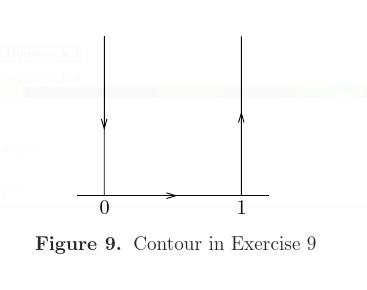
\includegraphics{figures/image_2020-06-17-21-52-40.png}
\end{quote}

\hypertarget{section-68}{%
\subsubsection{3.8.10}\label{section-68}}

Show that if \(a>0\), then
\begin{align*}
\int_{0}^{\infty} \frac{\log x}{x^{2}+a^{2}} d x=\frac{\pi}{2 a} \log a
.\end{align*}

\begin{quote}
Hint: use the following contour.

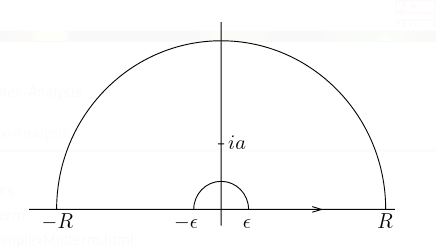
\includegraphics{figures/image_2020-06-17-21-53-19.png}
\end{quote}

\hypertarget{section-69}{%
\subsubsection{3.8.14}\label{section-69}}

Prove that all entire functions that are injective are of the form
\(f(z) = az + b\) with \(a,b\in {\mathbb{C}}\) and \(a\neq 0\).

\begin{quote}
Hint: Apply the Casorati-Weierstrass theorem to \(f(1/z)\).
\end{quote}

\hypertarget{section-70}{%
\subsubsection{3.8.15}\label{section-70}}

Use the Cauchy inequalities or the maximum modulus principle to solve
the following problems:

\begin{enumerate}
\def\labelenumi{\alph{enumi}.}
\item
  Prove that if \(f\) is an entire function that satisfies
  \begin{align*}
   \sup _{|z|=R}|f(z)| \leq A R^{k}+B
   \end{align*}
  for all \(R>0\), some integer \(k\geq 0\), and some constants
  \(A, B > 0\), then \(f\) is a polynomial of degree \(\leq k\).
\item
  Show that if \(f\) is holomorphic in the unit disc, is bounded, and
  converges uniformly to zero in the sector \(\theta < \arg(z) < \phi\)
  as \({\left\lvert {z} \right\rvert} \to 0\), then \(f \equiv 0\).
\item
  Let \(w_1, \cdots w_n\) be points on \(S^1 \subset {\mathbb{C}}\).
  Prove that there exists a point \(z\in S^1\) such that the product of
  the distances from \(z\) to the points \(w_j\) is at least 1.

  Conclude that there exists a point \(w\in S^1\) such that the product
  of the above distances is \emph{exactly} 1.
\item
  Show that if the real part of an entire function is bounded, then
  \(f\) is constant.
\end{enumerate}

\hypertarget{section-71}{%
\subsubsection{3.8.17}\label{section-71}}

Let \(f\) be non-constant and holomorphic in an open set containing the
closed unit disc.

\begin{enumerate}
\def\labelenumi{\alph{enumi}.}
\item
  Show that if \({\left\lvert {f(z)} \right\rvert} = 1\) whenever
  \({\left\lvert {z} \right\rvert} = 1\), then the image of \(f\)
  contains the unit disc.

  \begin{quote}
  Hint: Show that \(f(z) = w_0\) has a root for every
  \(w_0 \in {\mathbb{D}}\), for which it suffices to show that
  \(f(z) = 0\) has a root. Conclude using the maximum modulus principle.
  \end{quote}
\item
  If \({\left\lvert {f(z)} \right\rvert} \geq 1\) whenever
  \({\left\lvert {z} \right\rvert} = 1\) and there exists a
  \(z_0\in {\mathbb{D}}\) such that
  \({\left\lvert {f(z_0)} \right\rvert} < 1\), then the image of \(f\)
  contains the unit disc.
\end{enumerate}

\hypertarget{section-72}{%
\subsubsection{3.8.19}\label{section-72}}

Prove that maximum principle for harmonic functions, i.e.

\begin{enumerate}
\def\labelenumi{\alph{enumi}.}
\item
  If \(u\) is a non-constant real-valued harmonic function in a region
  \(\Omega\), then \(u\) can not attain a maximum or a minimum in
  \(\Omega\).
\item
  Suppose \(\Omega\) is a region with compact closure
  \(\mkern 1.5mu\overline{\mkern-1.5mu\Omega\mkern-1.5mu}\mkern 1.5mu\).
  If \(u\) is harmonic in \(\Omega\) and continuous in
  \(\mkern 1.5mu\overline{\mkern-1.5mu\Omega\mkern-1.5mu}\mkern 1.5mu\),
  then
  \begin{align*}
   \sup _{z \in \Omega}|u(z)| \leq \sup _{z \in \mkern 1.5mu\overline{\mkern-1.5mu\Omega \mkern-1.5mu}\mkern 1.5mu-\Omega}|u(z)|
   .\end{align*}
\end{enumerate}

\begin{quote}
Hint: to prove (a), assume \(u\) attains a local maximum at \(z_0\). Let
\(f\) be holomorphic near \(z_0\) with \(\Re(f) = u\), and show that
\(f\) is not an open map. Then (a) implies (b).
\end{quote}

\hypertarget{extra-problems}{%
\subsection{Extra Problems}\label{extra-problems}}

\hypertarget{section-73}{%
\subsubsection{1}\label{section-73}}

\begin{description}
\tightlist
\item[Problem]
Prove that if \(f\) has two Laurent series expansions,
\begin{align*}
  f(z) = \sum c_n(z-a)^n \quad\text{and}\quad f(z) = \sum c_n'(z-a)^n
  \end{align*}
then \(c_n = c_n'\).
\end{description}

\hypertarget{section-74}{%
\subsubsection{2}\label{section-74}}

\begin{description}
\tightlist
\item[Problem]
Find Laurent series expansions of
\begin{align*}
  \frac{1}{1-z^2} + \frac{1}{3-z}
  \end{align*}
How many such expansions are there? In what domains are each valid?
\end{description}

\hypertarget{section-75}{%
\subsubsection{3}\label{section-75}}

\begin{description}
\tightlist
\item[Problem]
Let \(P, Q\) be polynomials with no common zeros. Assume \(a\) is a root
of \(Q\). Find the principal part of \(P/Q\) at \(z=a\) in terms of
\(P\) and \(Q\) if \(a\) is (1) a simple root, and (2) a double root.
\end{description}

\hypertarget{section-76}{%
\subsubsection{4}\label{section-76}}

\begin{description}
\item[Problem]
Let \(f\) be non-constant, analytic in
\({\left\lvert {z} \right\rvert} > 0\), where \(f(z_n) = 0\) for
infinitely many points \(z_n\) with \(\lim_{n\to\infty} z_n = 0\).

Show that \(z=0\) is an essential singularity for \(f\).

\begin{quote}
Example: \(f(z) = \sin(1/z)\).
\end{quote}
\end{description}

\hypertarget{section-77}{%
\subsubsection{5}\label{section-77}}

\begin{description}
\tightlist
\item[Problem]
Show that if \(f\) is entire and \(\lim_{z\to\infty}f(z) = \infty\),
then \(f\) is a polynomial.
\end{description}

\hypertarget{section-78}{%
\subsubsection{6}\label{section-78}}

\begin{description}
\item[Problem]
\hfill

\begin{enumerate}
\def\labelenumi{\alph{enumi}.}
\tightlist
\item
  Show (without using 3.8.9 in the S\&S) that
  \begin{align*}
  \int_0^{2\pi} \log{\left\lvert {1 - e^{i\theta}} \right\rvert}~d\theta = 0
  \end{align*}
\item
  Show that this identity is equivalent to S\&S 3.8.9:
  \begin{align*}
  \int_0^1 \log(\sin(\pi x)) ~dx = -\log 2
  .\end{align*}
\end{enumerate}
\end{description}

\hypertarget{section-79}{%
\subsubsection{7}\label{section-79}}

\begin{description}
\tightlist
\item[Problem]
Let \(0<a<4\) and evaluate
\begin{align*}
  \int_0^\infty \frac{x^{\alpha-1}}{1+x^3} ~dx
  \end{align*}
\end{description}

\hypertarget{section-80}{%
\subsubsection{8}\label{section-80}}

\begin{description}
\item[Problem]
Prove the fundamental theorem of Algebra using

\begin{enumerate}
\def\labelenumi{\alph{enumi}.}
\tightlist
\item
  Rouche's Theorem.
\item
  The maximum modulus principle.
\end{enumerate}
\end{description}

\hypertarget{section-81}{%
\subsubsection{9}\label{section-81}}

\begin{description}
\item[Problem]
Let \(f\) be analytic in a region \(D\) and \(\gamma\) a rectifiable
curve in \(D\) with interior in \(D\).

Prove that if \(f(z)\) is real for all \(z\in \gamma\), then \(f\) is
constant.
\end{description}

\hypertarget{section-82}{%
\subsubsection{10}\label{section-82}}

\begin{description}
\tightlist
\item[Problem]
For \(a> 0\), evaluate
\begin{align*}
  \int_0^{\pi/2} \frac{d\theta}{a + \sin^2 \theta}
  \end{align*}
\end{description}

\hypertarget{section-83}{%
\subsubsection{11}\label{section-83}}

\begin{description}
\tightlist
\item[Problem]
Find the number of roots of \(p(z) = 4z^4 - 6z + 3\) in
\({\left\lvert {z} \right\rvert} < 1\) and
\(1 < {\left\lvert {z} \right\rvert} < 2\) respectively.
\end{description}

\hypertarget{section-84}{%
\subsubsection{12}\label{section-84}}

\begin{description}
\tightlist
\item[Problem]
Prove that \(z^4 + 2z^3 -2z + 10\) has exactly one root in each open
quadrant.
\end{description}

\hypertarget{section-85}{%
\subsubsection{13}\label{section-85}}

\begin{description}
\tightlist
\item[Problem]
Prove that for \(a> 0\), \(z\tan z - a\) has only real roots.
\end{description}

\hypertarget{section-86}{%
\subsubsection{14}\label{section-86}}

\begin{description}
\item[Problem]
Let \(f\) be nonzero, analytic on a bounded region \(\Omega\) and
continuous on its closure \(\overline \Omega\).

Show that if \({\left\lvert {f(z)} \right\rvert} \equiv M\) is constant
for \(z\in \partial \Omega\), then \(f(z) \equiv Me^{i\theta}\) for some
real constant \(\theta\).
\end{description}

\hypertarget{extra-questions-from-jingzhi-tie}{%
\section{Extra Questions from Jingzhi
Tie}\label{extra-questions-from-jingzhi-tie}}

\hypertarget{fall-2009}{%
\subsection{Fall 2009}\label{fall-2009}}

\hypertarget{section-87}{%
\subsubsection{?}\label{section-87}}

\begin{enumerate}
\def\labelenumi{(\arabic{enumi})}
\item
  Assume \(\displaystyle f(z) = \sum_{n=0}^\infty c_n z^n\) converges in
  \(|z| < R\). Show that for \(r <R\),
  \begin{align*}\frac{1}{2 \pi} \int_0^{2 \pi} |f(r e^{i \theta})|^2 d \theta =
  \sum_{n=0}^\infty |c_n|^2 r^{2n} \; .\end{align*}
\item
  Deduce Liouville's theorem from (1).
\end{enumerate}

\hypertarget{section-88}{%
\subsubsection{?}\label{section-88}}

Let \(f\) be a continuous function in the region
\begin{align*}D=\{z {~\mathrel{\Big|}~}{\left\lvert {z} \right\rvert}>R, 0\leq \arg z\leq \theta\}\quad\text{where}\quad
1\leq \theta \leq 2\pi.\end{align*}
If there exists \(k\) such that
\(\displaystyle{\lim_{z\to\infty} zf(z)=k}\) for \(z\) in the region
\(D\). Show that
\begin{align*}\lim_{R'\to\infty} \int_{L} f(z) dz=i\theta k,\end{align*}
where \(L\) is the part of the circle \(|z|=R'\) which lies in the
region \(D\).

\hypertarget{section-89}{%
\subsubsection{?}\label{section-89}}

Suppose that \(f\) is an analytic function in the region \(D\) which
contains the point \(a\). Let
\begin{align*}F(z)= z-a-qf(z),\quad \text{where}~ q \ \text{is a complex
parameter}.\end{align*}

\begin{enumerate}
\def\labelenumi{(\arabic{enumi})}
\item
  Let \(K\subset D\) be a circle with the center at point \(a\) and also
  we assume that \(f(z)\not =0\) for \(z\in K\). Prove that the function
  \(F\) has one and only one zero \(z=w\) on the closed disc
  \(\mkern 1.5mu\overline{\mkern-1.5muK\mkern-1.5mu}\mkern 1.5mu\) whose
  boundary is the circle \(K\) if
  \(\displaystyle{ |q|<\min_{z\in K} \frac{|z-a|}{|f(z)|}.}\)\\
\item
  Let \(G(z)\) be an analytic function on the disk
  \(\mkern 1.5mu\overline{\mkern-1.5muK\mkern-1.5mu}\mkern 1.5mu\).
  Apply the residue theorem to prove that
  \(\displaystyle{ \frac{G(w)}{F'(w)}=\frac{1}{2\pi i}\int_K \frac{G(z)}{F(z)} dz,}\)
  where \(w\) is the zero from (1).\\
\item
  If \(z\in K\), prove that the function
  \(\displaystyle{\frac{1}{F(z)}}\) can be represented as a convergent
  series with respect to \(q\):
  \(\displaystyle{ \frac{1}{F(z)}=\sum_{n=0}^{\infty} \frac{(qf(z))^n}{(z-a)^{n+1}}.}\)
\end{enumerate}

\hypertarget{section-90}{%
\subsubsection{?}\label{section-90}}

Evaluate
\begin{align*}\displaystyle{ \int_{0}^{\infty}\frac{x\sin x}{x^2+a^2} \,
dx }.\end{align*}

\hypertarget{section-91}{%
\subsubsection{?}\label{section-91}}

Let \(f=u+iv\) be differentiable (i.e.~\(f'(z)\) exists) with continuous
partial derivatives at a point \(z=re^{i\theta}\), \(r\not= 0\). Show
that
\begin{align*}\frac{\partial u}{\partial r}=\frac{1}{r}\frac{\partial v}{\partial \theta},\quad
\frac{\partial v}{\partial r}=-\frac{1}{r}\frac{\partial u}{\partial \theta}.\end{align*}

\hypertarget{section-92}{%
\subsubsection{?}\label{section-92}}

Show that
\(\displaystyle \int_0^\infty \frac{x^{a-1}}{1+x^n} dx=\frac{\pi}{n\sin \frac{a\pi}{n}}\)
using complex analysis, \(0< a < n\). Here \(n\) is a positive integer.

\hypertarget{section-93}{%
\subsubsection{?}\label{section-93}}

For \(s>0\), the \textbf{gamma function} is defined by
\(\displaystyle{\Gamma(s)=\int_0^{\infty} e^{-t}t^{s-1} dt}\).

\begin{enumerate}
\def\labelenumi{\arabic{enumi}.}
\item
  Show that the gamma function is analytic in the half-plane
  \(\Re (s)>0\), and is still given there by the integral formula above.
\item
  Apply the formula in the previous question to show that
  \begin{align*}\Gamma(s)\Gamma(1-s)=\frac{\pi}{\sin \pi s}.\end{align*}
\end{enumerate}

\begin{quote}
Hint: You may need
\(\displaystyle{\Gamma(1-s)=t \int_0^{\infty}e^{-vt}(vt)^{-s} dv}\) for
\(t>0\).
\end{quote}

\hypertarget{section-94}{%
\subsubsection{?}\label{section-94}}

Apply Rouché's Theorem to prove the Fundamental Theorem of Algebra: If
\begin{align*}P_n(z) = a_0 + a_1z + \cdots + a_{n-1}z^{n-1} + a_nz^n\quad  (a_n \neq 0)\end{align*}
is a polynomial of degree n, then it has n zeros in \(\mathbb C\).

\hypertarget{section-95}{%
\subsubsection{?}\label{section-95}}

Suppose \(f\) is entire and there exist \(A, R >0\) and natural number
\(N\) such that
\begin{align*}|f(z)| \geq A |z|^N\ \text{for}\ |z| \geq R.\end{align*}
Show that (i) \(f\) is a polynomial and (ii) the degree of \(f\) is at
least \(N\).

\hypertarget{section-96}{%
\subsubsection{?}\label{section-96}}

Let \(f: {\mathbb C} \rightarrow {\mathbb C}\) be an injective analytic
(also called \emph{univalent}) function. Show that there exist complex
numbers \(a \neq 0\) and \(b\) such that \(f(z) = az + b\).

\hypertarget{section-97}{%
\subsubsection{?}\label{section-97}}

Let \(g\) be analytic for \(|z|\leq 1\) and \(|g(z)| < 1\) for
\(|z| = 1\).

\begin{enumerate}
\def\labelenumi{\arabic{enumi}.}
\item
  Show that \(g\) has a unique fixed point in \(|z| < 1\).
\item
  What happens if we replace \(|g(z)| < 1\) with \(|g(z)|\leq 1\) for
  \(|z|=1\)? Give an example if (a) is not true or give an proof if (a)
  is still true.
\item
  What happens if we simply assume that \(f\) is analytic for
  \(|z| < 1\) and \(|f(z)| < 1\) for \(|z| < 1\)? Suppose that
  \(f(z) \not\equiv z\). Can f have more than one fixed point in
  \(|z| < 1\)?
\end{enumerate}

\begin{quote}
Hint: The map
\(\displaystyle{\psi_{\alpha}(z)=\frac{\alpha-z}{1-\mkern 1.5mu\overline{\mkern-1.5mu\alpha\mkern-1.5mu}\mkern 1.5muz}}\)
may be useful.
\end{quote}

\hypertarget{section-98}{%
\subsubsection{?}\label{section-98}}

Find a conformal map from \(D = \{z :\  |z| < 1,\ |z - 1/2| > 1/2\}\) to
the unit disk \(\Delta=\{z: \ |z|<1\}\).

\hypertarget{section-99}{%
\subsubsection{?}\label{section-99}}

Let \(f(z)\) be entire and assume values of \(f(z)\) lie outside a
\emph{bounded} open set \(\Omega\). Show without using Picard's theorems
that \(f(z)\) is a constant.

\hypertarget{section-100}{%
\subsubsection{?}\label{section-100}}

\begin{enumerate}
\def\labelenumi{(\arabic{enumi})}
\item
  Assume \(\displaystyle f(z) = \sum_{n=0}^\infty c_n z^n\) converges in
  \(|z| < R\). Show that for \(r <R\),
  \begin{align*}\frac{1}{2 \pi} \int_0^{2 \pi} |f(r e^{i \theta})|^2 d \theta
  = \sum_{n=0}^\infty |c_n|^2 r^{2n} \; .\end{align*}
\item
  Deduce Liouville's theorem from (1).
\end{enumerate}

\hypertarget{section-101}{%
\subsubsection{?}\label{section-101}}

Let \(f(z)\) be entire and assume that \(f(z) \leq M |z|^2\) outside
some disk for some constant \(M\). Show that \(f(z)\) is a polynomial in
\(z\) of degree \(\leq 2\).

\hypertarget{section-102}{%
\subsubsection{?}\label{section-102}}

Let \(a_n(z)\) be an analytic sequence in a domain \(D\) such that
\(\displaystyle \sum_{n=0}^\infty |a_n(z)|\) converges uniformly on
bounded and closed sub-regions of \(D\). Show that
\(\displaystyle \sum_{n=0}^\infty |a'_n(z)|\) converges uniformly on
bounded and closed sub-regions of \(D\).

\hypertarget{section-103}{%
\subsubsection{?}\label{section-103}}

Let \(f(z)\) be analytic in an open set \(\Omega\) except possibly at a
point \(z_0\) inside \(\Omega\). Show that if \(f(z)\) is bounded in
near \(z_0\), then \(\displaystyle \int_\Delta f(z) dz = 0\) for all
triangles \(\Delta\) in \(\Omega\).

\hypertarget{section-104}{%
\subsubsection{?}\label{section-104}}

Assume \(f\) is continuous in the region:
\(0< |z-a| \leq R, \; 0 \leq \arg(z-a) \leq \beta_0\)
(\(0 < \beta_0 \leq 2 \pi\)) and the limit
\(\displaystyle \lim_{z \rightarrow a} (z-a) f(z) = A\) exists. Show
that
\begin{align*}\lim_{r \rightarrow 0} \int_{\gamma_r} f(z) dz  = i A \beta_0 \; , \; \;\end{align*}
where
\(\gamma_r : = \{ z \; | \; z = a + r e^{it}, \; 0 \leq t \leq \beta_0 \}.\)

\hypertarget{section-105}{%
\subsubsection{?}\label{section-105}}

Show that \(f(z) = z^2\) is uniformly continuous in any open disk
\(|z| < R\), where \(R>0\) is fixed, but it is not uniformly continuous
on \(\mathbb C\).

\hypertarget{section-106}{%
\subsubsection{?}\label{section-106}}

\begin{enumerate}
\def\labelenumi{(\arabic{enumi})}
\tightlist
\item
  Show that the function \(u=u(x,y)\) given by
  \begin{align*}u(x,y)=\frac{e^{ny}-e^{-ny}}{2n^2}\sin nx\quad \text{for}\ n\in {\mathbf N}\end{align*}
  is the solution on \(D=\{(x,y)\ | x^2+y^2<1\}\) of the Cauchy problem
  for the Laplace equation
  \begin{align*}\frac{\partial ^2u}{\partial x^2}+\frac{\partial ^2u}{\partial y^2}=0,\quad
  u(x,0)=0,\quad \frac{\partial u}{\partial y}(x,0)=\frac{\sin nx}{n}.\end{align*}
\item
  Show that there exist points \((x,y)\in D\) such that
  \(\displaystyle{\limsup_{n\to\infty} |u(x,y)|=\infty}\).
\end{enumerate}

\hypertarget{fall-2011}{%
\subsection{Fall 2011}\label{fall-2011}}

\hypertarget{section-107}{%
\subsubsection{?}\label{section-107}}

\begin{enumerate}
\def\labelenumi{(\arabic{enumi})}
\item
  Assume \(\displaystyle f(z) = \sum_{n=0}^\infty c_n z^n\) converges in
  \(|z| < R\). Show that for \(r <R\),
  \begin{align*}\frac{1}{2 \pi} \int_0^{2 \pi} |f(r e^{i \theta})|^2 d \theta =
  \sum_{n=0}^\infty |c_n|^2 r^{2n} \; .\end{align*}
\item
  Deduce Liouville's theorem from (1).
\end{enumerate}

\hypertarget{section-108}{%
\subsubsection{?}\label{section-108}}

Let \(f\) be a continuous function in the region
\begin{align*}D=\{z\ |  |z|>R, 0\leq \arg Z\leq \theta\}\quad\text{where}\quad
0\leq \theta \leq 2\pi.\end{align*}
If there exists \(k\) such that
\(\displaystyle{\lim_{z\to\infty} zf(z)=k}\) for \(z\) in the region
\(D\). Show that
\begin{align*}\lim_{R'\to\infty} \int_{L} f(z) dz=i\theta k,\end{align*}
where \(L\) is the part of the circle \(|z|=R'\) which lies in the
region \(D\).

\hypertarget{section-109}{%
\subsubsection{?}\label{section-109}}

Suppose that \(f\) is an analytic function in the region \(D\) which
contains the point \(a\). Let
\begin{align*}F(z)= z-a-qf(z),\quad \text{where}\quad q \ \text{is a complex
parameter}.\end{align*}

\begin{enumerate}
\def\labelenumi{(\arabic{enumi})}
\item
  Let \(K\subset D\) be a circle with the center at point \(a\) and also
  we assume that \(f(z)\not =0\) for \(z\in K\). Prove that the function
  \(F\) has one and only one zero \(z=w\) on the closed disc
  \(\mkern 1.5mu\overline{\mkern-1.5muK\mkern-1.5mu}\mkern 1.5mu\) whose
  boundary is the circle \(K\) if
  \(\displaystyle{ |q|<\min_{z\in K} \frac{|z-a|}{|f(z)|}.}\)\\
\item
  Let \(G(z)\) be an analytic function on the disk
  \(\mkern 1.5mu\overline{\mkern-1.5muK\mkern-1.5mu}\mkern 1.5mu\).
  Apply the residue theorem to prove that
  \(\displaystyle{ \frac{G(w)}{F'(w)}=\frac{1}{2\pi i}\int_K \frac{G(z)}{F(z)} dz,}\)
  where \(w\) is the zero from (1).\\
\item
  If \(z\in K\), prove that the function
  \(\displaystyle{\frac{1}{F(z)}}\) can be represented as a convergent
  series with respect to \(q\):
  \(\displaystyle{ \frac{1}{F(z)}=\sum_{n=0}^{\infty} \frac{(qf(z))^n}{(z-a)^{n+1}}.}\)
\end{enumerate}

\hypertarget{section-110}{%
\subsubsection{?}\label{section-110}}

Evaluate
\(\displaystyle{ \int_{0}^{\infty}\frac{x\sin x}{x^2+a^2} \, dx }\).

\hypertarget{section-111}{%
\subsubsection{?}\label{section-111}}

Let \(f=u+iv\) be differentiable (i.e.~\(f'(z)\) exists) with continuous
partial derivatives at a point \(z=re^{i\theta}\), \(r\not= 0\). Show
that
\begin{align*}\frac{\partial u}{\partial r}=\frac{1}{r}\frac{\partial v}{\partial \theta},\quad
\frac{\partial v}{\partial r}=-\frac{1}{r}\frac{\partial u}{\partial \theta}.\end{align*}

\hypertarget{section-112}{%
\subsubsection{?}\label{section-112}}

Show that
\(\displaystyle \int_0^\infty \frac{x^{a-1}}{1+x^n} dx=\frac{\pi}{n\sin \frac{a\pi}{n}}\)
using complex analysis, \(0< a < n\). Here \(n\) is a positive integer.

\hypertarget{section-113}{%
\subsubsection{?}\label{section-113}}

For \(s>0\), the \textbf{gamma function} is defined by
\(\displaystyle{\Gamma(s)=\int_0^{\infty} e^{-t}t^{s-1} dt}\).

\begin{enumerate}
\def\labelenumi{\arabic{enumi}.}
\item
  Show that the gamma function is analytic in the half-plane
  \(\Re (s)>0\), and is still given there by the integral formula above.
\item
  Apply the formula in the previous question to show that
  \begin{align*}\Gamma(s)\Gamma(1-s)=\frac{\pi}{\sin \pi s}.\end{align*}
\end{enumerate}

\begin{quote}
Hint: You may need
\(\displaystyle{\Gamma(1-s)=t \int_0^{\infty}e^{-vt}(vt)^{-s} dv}\) for
\(t>0\).
\end{quote}

\hypertarget{section-114}{%
\subsubsection{?}\label{section-114}}

Apply Rouché's Theorem to prove the Fundamental Theorem of Algebra: If
\begin{align*}P_n(z) = a_0 + a_1z + \cdots + a_{n-1}z^{n-1} + a_nz^n\quad  (a_n \neq 0)\end{align*}
is a polynomial of degree n, then it has n zeros in \(\mathbb C\).

\hypertarget{section-115}{%
\subsubsection{?}\label{section-115}}

Suppose \(f\) is entire and there exist \(A, R >0\) and natural number
\(N\) such that
\begin{align*}|f(z)| \geq A |z|^N\ \text{for}\ |z| \geq R.\end{align*}
Show that (i) \(f\) is a polynomial and (ii) the degree of \(f\) is at
least \(N\).

\hypertarget{section-116}{%
\subsubsection{?}\label{section-116}}

Let \(f: {\mathbb C} \rightarrow {\mathbb C}\) be an injective analytic
(also called univalent) function. Show that there exist complex numbers
\(a \neq 0\) and \(b\) such that \(f(z) = az + b\).

\hypertarget{section-117}{%
\subsubsection{?}\label{section-117}}

Let \(g\) be analytic for \(|z|\leq 1\) and \(|g(z)| < 1\) for
\(|z| = 1\).

\begin{itemize}
\item
  Show that \(g\) has a unique fixed point in \(|z| < 1\).
\item
  What happens if we replace \(|g(z)| < 1\) with \(|g(z)|\leq 1\) for
  \(|z|=1\)? Give an example if (a) is not true or give an proof if (a)
  is still true.
\item
  What happens if we simply assume that \(f\) is analytic for
  \(|z| < 1\) and \(|f(z)| < 1\) for \(|z| < 1\)? Suppose that
  \(f(z) \not\equiv z\). Can f have more than one fixed point in
  \(|z| < 1\)?
\end{itemize}

\begin{quote}
Hint: The map
\(\displaystyle{\psi_{\alpha}(z)=\frac{\alpha-z}{1-\mkern 1.5mu\overline{\mkern-1.5mu\alpha\mkern-1.5mu}\mkern 1.5muz}}\)
may be useful.
\end{quote}

\hypertarget{section-118}{%
\subsubsection{?}\label{section-118}}

Find a conformal map from \(D = \{z :\  |z| < 1,\ |z - 1/2| > 1/2\}\) to
the unit disk \(\Delta=\{z: \ |z|<1\}\).

\hypertarget{section-119}{%
\subsubsection{?}\label{section-119}}

Let \(f(z)\) be entire and assume values of \(f(z)\) lie outside a
\emph{bounded} open set \(\Omega\). Show without using Picard's theorems
that \(f(z)\) is a constant.

\hypertarget{section-120}{%
\subsubsection{?}\label{section-120}}

Let \(f(z)\) be entire and assume values of \(f(z)\) lie outside a
\emph{bounded} open set \(\Omega\). Show without using Picard's theorems
that \(f(z)\) is a constant.

\hypertarget{section-121}{%
\subsubsection{?}\label{section-121}}

\begin{enumerate}
\def\labelenumi{(\arabic{enumi})}
\item
  Assume \(\displaystyle f(z) = \sum_{n=0}^\infty c_n z^n\) converges in
  \(|z| < R\). Show that for \(r <R\),
  \begin{align*}\frac{1}{2 \pi} \int_0^{2 \pi} |f(r e^{i \theta})|^2 d \theta
  = \sum_{n=0}^\infty |c_n|^2 r^{2n} \; .\end{align*}
\item
  Deduce Liouville's theorem from (1).
\end{enumerate}

\hypertarget{section-122}{%
\subsubsection{?}\label{section-122}}

Let \(f(z)\) be entire and assume that \(f(z) \leq M |z|^2\) outside
some disk for some constant \(M\). Show that \(f(z)\) is a polynomial in
\(z\) of degree \(\leq 2\).

\hypertarget{section-123}{%
\subsubsection{?}\label{section-123}}

Let \(a_n(z)\) be an analytic sequence in a domain \(D\) such that
\(\displaystyle \sum_{n=0}^\infty |a_n(z)|\) converges uniformly on
bounded and closed sub-regions of \(D\). Show that
\(\displaystyle \sum_{n=0}^\infty |a'_n(z)|\) converges uniformly on
bounded and closed sub-regions of \(D\).

\hypertarget{section-124}{%
\subsubsection{?}\label{section-124}}

Let \(f(z)\) be analytic in an open set \(\Omega\) except possibly at a
point \(z_0\) inside \(\Omega\). Show that if \(f(z)\) is bounded in
near \(z_0\), then \(\displaystyle \int_\Delta f(z) dz = 0\) for all
triangles \(\Delta\) in \(\Omega\).

\hypertarget{section-125}{%
\subsubsection{?}\label{section-125}}

Assume \(f\) is continuous in the region:
\(0< |z-a| \leq R, \; 0 \leq \arg(z-a) \leq \beta_0\)
(\(0 < \beta_0 \leq 2 \pi\)) and the limit
\(\displaystyle \lim_{z \rightarrow a} (z-a) f(z) = A\) exists. Show
that
\begin{align*}\lim_{r \rightarrow 0} \int_{\gamma_r} f(z) dz  = i A \beta_0 \; , \; \;\end{align*}
where
\(\gamma_r : = \{ z \; | \; z = a + r e^{it}, \; 0 \leq t \leq \beta_0 \}.\)

\hypertarget{section-126}{%
\subsubsection{?}\label{section-126}}

Show that \(f(z) = z^2\) is uniformly continuous in any open disk
\(|z| < R\), where \(R>0\) is fixed, but it is not uniformly continuous
on \(\mathbb C\).

\begin{enumerate}
\def\labelenumi{(\arabic{enumi})}
\tightlist
\item
  Show that the function \(u=u(x,y)\) given by
  \begin{align*}u(x,y)=\frac{e^{ny}-e^{-ny}}{2n^2}\sin nx\quad \text{for}\ n\in {\mathbf N}\end{align*}
  is the solution on \(D=\{(x,y)\ | x^2+y^2<1\}\) of the Cauchy problem
  for the Laplace equation
  \begin{align*}\frac{\partial ^2u}{\partial x^2}+\frac{\partial ^2u}{\partial y^2}=0,\quad
  u(x,0)=0,\quad \frac{\partial u}{\partial y}(x,0)=\frac{\sin nx}{n}.\end{align*}
\item
  Show that there exist points \((x,y)\in D\) such that
  \(\displaystyle{\limsup_{n\to\infty} |u(x,y)|=\infty}\).
\end{enumerate}

\hypertarget{spring-2014}{%
\subsection{Spring 2014}\label{spring-2014}}

\hypertarget{section-127}{%
\subsubsection{?}\label{section-127}}

The question provides some insight into Cauchy's theorem. Solve the
problem without using the Cauchy theorem.

\begin{enumerate}
\def\labelenumi{\arabic{enumi}.}
\item
  Evaluate the integral \(\displaystyle{\int_{\gamma} z^n dz}\) for all
  integers \(n\). Here \(\gamma\) is any circle centered at the origin
  with the positive (counterclockwise) orientation.
\item
  Same question as (a), but with \(\gamma\) any circle not containing
  the origin.
\item
  Show that if \(|a|<r<|b|\), then
  \(\displaystyle{\int_{\gamma}\frac{dz}{(z-a)(z-b)} dz=\frac{2\pi i}{a-b}}\).
  Here \(\gamma\) denotes the circle centered at the origin, of radius
  \(r\), with the positive orientation.
\end{enumerate}

\hypertarget{section-128}{%
\subsubsection{?}\label{section-128}}

\begin{enumerate}
\def\labelenumi{(\arabic{enumi})}
\item
  Assume the infinite series \(\displaystyle \sum_{n=0}^\infty c_n z^n\)
  converges in \(|z| < R\) and let \(f(z)\) be the limit. Show that for
  \(r <R\),
  \begin{align*}\frac{1}{2 \pi} \int_0^{2 \pi} |f(r e^{i \theta})|^2 d \theta =
  \sum_{n=0}^\infty |c_n|^2 r^{2n} \; .\end{align*}
\item
  Deduce Liouville's theorem from (1). Liouville's theorem: If \(f(z)\)
  is entire and bounded, then \(f\) is constant.
\end{enumerate}

\hypertarget{section-129}{%
\subsubsection{?}\label{section-129}}

Let \(f\) be a continuous function in the region
\begin{align*}D=\{z\ |  |z|>R, 0\leq \arg Z\leq \theta\}\quad\text{where}\quad
0\leq \theta \leq 2\pi.\end{align*}
If there exists \(k\) such that
\(\displaystyle{\lim_{z\to\infty} zf(z)=k}\) for \(z\) in the region
\(D\). Show that
\begin{align*}\lim_{R'\to\infty} \int_{L} f(z) dz=i\theta k,\end{align*}
where \(L\) is the part of the circle \(|z|=R'\) which lies in the
region \(D\).

\hypertarget{section-130}{%
\subsubsection{?}\label{section-130}}

Evaluate
\(\displaystyle{ \int_{0}^{\infty}\frac{x\sin x}{x^2+a^2} \, dx }\).

\hypertarget{section-131}{%
\subsubsection{?}\label{section-131}}

Let \(f=u+iv\) be differentiable (i.e.~\(f'(z)\) exists) with continuous
partial derivatives at a point \(z=re^{i\theta}\), \(r\not= 0\). Show
that
\begin{align*}\frac{\partial u}{\partial r}=\frac{1}{r}\frac{\partial v}{\partial \theta},\quad
\frac{\partial v}{\partial r}=-\frac{1}{r}\frac{\partial u}{\partial \theta}.\end{align*}

\hypertarget{section-132}{%
\subsubsection{?}\label{section-132}}

Show that
\(\displaystyle \int_0^\infty \frac{x^{a-1}}{1+x^n} dx=\frac{\pi}{n\sin \frac{a\pi}{n}}\)
using complex analysis, \(0< a < n\). Here \(n\) is a positive integer.

\hypertarget{section-133}{%
\subsubsection{?}\label{section-133}}

For \(s>0\), the \textbf{gamma function} is defined by
\(\displaystyle{\Gamma(s)=\int_0^{\infty} e^{-t}t^{s-1} dt}\).

\begin{itemize}
\item
  Show that the gamma function is analytic in the half-plane
  \(\Re (s)>0\), and is still given there by the integral formula above.
\item
  Apply the formula in the previous question to show that
  \begin{align*}\Gamma(s)\Gamma(1-s)=\frac{\pi}{\sin \pi s}.\end{align*}
\end{itemize}

\begin{quote}
Hint: You may need
\(\displaystyle{\Gamma(1-s)=t \int_0^{\infty}e^{-vt}(vt)^{-s} dv}\) for
\(t>0\).
\end{quote}

\hypertarget{section-134}{%
\subsubsection{?}\label{section-134}}

Apply Rouché's Theorem to prove the Fundamental Theorem of Algebra: If
\begin{align*}P_n(z) = a_0 + a_1z + \cdots + a_{n-1}z^{n-1} + a_nz^n\quad  (a_n \neq 0)\end{align*}
is a polynomial of degree n, then it has n zeros in \(\mathbf C\).

\hypertarget{section-135}{%
\subsubsection{?}\label{section-135}}

Suppose \(f\) is entire and there exist \(A, R >0\) and natural number
\(N\) such that
\begin{align*}|f(z)| \geq A |z|^N\ \text{for}\ |z| \geq R.\end{align*}
Show that (i) \(f\) is a polynomial and (ii) the degree of \(f\) is at
least \(N\).

\hypertarget{section-136}{%
\subsubsection{?}\label{section-136}}

Let \(f: {\mathbb C} \rightarrow {\mathbb C}\) be an injective analytic
(also called univalent) function. Show that there exist complex numbers
\(a \neq 0\) and \(b\) such that \(f(z) = az + b\).

\hypertarget{section-137}{%
\subsubsection{?}\label{section-137}}

Let \(g\) be analytic for \(|z|\leq 1\) and \(|g(z)| < 1\) for
\(|z| = 1\).

\begin{itemize}
\item
  Show that \(g\) has a unique fixed point in \(|z| < 1\).
\item
  What happens if we replace \(|g(z)| < 1\) with \(|g(z)|\leq 1\) for
  \(|z|=1\)? Give an example if (a) is not true or give an proof if (a)
  is still true.
\item
  What happens if we simply assume that \(f\) is analytic for
  \(|z| < 1\) and \(|f(z)| < 1\) for \(|z| < 1\)? Suppose that
  \(f(z) \not\equiv z\). Can f have more than one fixed point in
  \(|z| < 1\)?
\end{itemize}

\begin{quote}
Hint: The map
\(\displaystyle{\psi_{\alpha}(z)=\frac{\alpha-z}{1-\mkern 1.5mu\overline{\mkern-1.5mu\alpha\mkern-1.5mu}\mkern 1.5muz}}\)
may be useful.
\end{quote}

\hypertarget{section-138}{%
\subsubsection{?}\label{section-138}}

Find a conformal map from \(D = \{z :\  |z| < 1,\ |z - 1/2| > 1/2\}\) to
the unit disk \(\Delta=\{z: \ |z|<1\}\).

\hypertarget{fall-2015}{%
\subsection{Fall 2015}\label{fall-2015}}

\hypertarget{section-139}{%
\subsubsection{?}\label{section-139}}

Let \(a_n \neq 0\) and assume that
\(\displaystyle \lim_{n \rightarrow \infty} \frac{|a_{n+1}|}{|a_n|} = L\).
Show that
\(\displaystyle \lim_{n \rightarrow \infty} \sqrt[n]{|a_n|} = L. %p_n^{\frac{1}{n}} = L.
\) In particular, this shows that when applicable, the ratio test can be
used to calculate the radius of convergence of a power series.

\hypertarget{section-140}{%
\subsubsection{?}\label{section-140}}

\begin{enumerate}
\def\labelenumi{(\alph{enumi})}
\item
  Let \(z, w\) be complex numbers, such that
  \(\mkern 1.5mu\overline{\mkern-1.5muz\mkern-1.5mu}\mkern 1.5mu w \neq 1\).
  Prove that
  \begin{align*}{\left\lvert {\frac{w - z}{1 - \mkern 1.5mu\overline{\mkern-1.5muw\mkern-1.5mu}\mkern 1.5mu z}} \right\rvert} < 1 \; \; \; \mbox{if} \; |z| < 1 \; \mbox{and}\; |w| < 1,\end{align*}
  and also that
  \begin{align*}{\left\lvert {\frac{w - z}{1 - \mkern 1.5mu\overline{\mkern-1.5muw\mkern-1.5mu}\mkern 1.5mu z}} \right\rvert} = 1 \; \; \; \mbox{if} \; |z| = 1 \; \mbox{or}\; |w| = 1.\end{align*}
\item
  Prove that for fixed \(w\) in the unit disk \(\mathbb D\), the mapping
  \begin{align*}F: z \mapsto \frac{w - z}{1 - \mkern 1.5mu\overline{\mkern-1.5muw\mkern-1.5mu}\mkern 1.5mu z}\end{align*}
  satisfies the following conditions:
\item
  \(F\) maps \(\mathbb D\) to itself and is holomorphic.~
\end{enumerate}

\begin{enumerate}
\def\labelenumi{(\roman{enumi})}
\setcounter{enumi}{1}
\item
  \(F\) interchanges \(0\) and \(w\), namely, \(F(0) = w\) and
  \(F(w) = 0\).
\item
  \(|F(z)| = 1\) if \(|z| = 1\).
\item
  \(F: {\mathbb D} \mapsto {\mathbb D}\) is bijective.
\end{enumerate}

\begin{quote}
Hint: Calculate \(F \circ F\).
\end{quote}

\hypertarget{section-141}{%
\subsubsection{?}\label{section-141}}

Use \(n\)-th roots of unity (i.e.~solutions of \(z^n - 1 =0\)) to show
that
\begin{align*}2^{n-1} \sin\frac{\pi}{n} \sin\frac{2\pi}{n} \cdots \sin\frac{(n-1)\pi}{n}
= n
\; .\end{align*}

\begin{quote}
Hint:
\(1 - \cos 2 \theta = 2 \sin^2 \theta,\; \sin 2 \theta = 2 \sin \theta \cos \theta\).
\end{quote}

\begin{enumerate}
\def\labelenumi{(\alph{enumi})}
\tightlist
\item
  Show that in polar coordinates, the Cauchy-Riemann equations take the
  form
\end{enumerate}

\begin{align*}\frac{\partial u}{\partial r} = \frac{1}{r} \frac{\partial v}{\partial \theta}
\; \; \; \text{and} \; \; \;
\frac{\partial v}{\partial r} = - \frac{1}{r} \frac{\partial u}{\partial \theta}\end{align*}

\begin{enumerate}
\def\labelenumi{(\alph{enumi})}
\setcounter{enumi}{1}
\tightlist
\item
  Use these equations to show that the logarithm function defined by
  \begin{align*}\log z = \log r + i \theta \; \;
  \mbox{where} \; z = r e^{i \theta } \; \mbox{with} \; - \pi < \theta < \pi\end{align*}
  is a holomorphic function in the region
  \(r>0, \; - \pi < \theta < \pi\). Also show that \(\log z\) defined
  above is not continuous in \(r>0\).
\end{enumerate}

\hypertarget{section-142}{%
\subsubsection{?}\label{section-142}}

Assume \(f\) is continuous in the region:
\(x \geq x_0, \; 0 \leq y \leq b\) and the limit
\begin{align*}\displaystyle \lim_{x \rightarrow + \infty} f(x + iy) = A\end{align*}
exists uniformly with respect to \(y\) (independent of \(y\)). Show that
\begin{align*}\lim_{x \rightarrow + \infty} \int_{\gamma_x} f(z) dz  = iA b \; , \; \;\end{align*}
where \(\gamma_x : = \{ z \; | \; z = x + it, \; 0 \leq t \leq b\}.\)

\hypertarget{section-143}{%
\subsubsection{?}\label{section-143}}

(Cauchy's formula for ``exterior'' region) Let \(\gamma\) be piecewise
smooth simple closed curve with interior \(\Omega_1\) and exterior
\(\Omega_2\). Assume \(f'(z)\) exists in an open set containing
\(\gamma\) and \(\Omega_2\) and
\(\lim_{z \rightarrow \infty } f(z) = A\). Show that
\begin{align*}\frac{1}{2 \pi i} \int_\gamma \frac{f(\xi)}{\xi - z} \, d \xi =
\begin{cases}
A,          &     \text{if\ $z \in \Omega_1$}, \\
-f (z) + A, &  \text{if\ $z \in \Omega_2$}
\end{cases}\end{align*}

\hypertarget{section-144}{%
\subsubsection{?}\label{section-144}}

Let \(f(z)\) be bounded and analytic in \(\mathbb C\). Let \(a \neq b\)
be any fixed complex numbers. Show that the following limit exists
\begin{align*}\lim_{R \rightarrow \infty} \int_{|z|=R} \frac{f(z)}{(z-a)(z-b)} dz.\end{align*}
Use this to show that \(f(z)\) must be a constant (Liouville's theorem).

\hypertarget{section-145}{%
\subsubsection{?}\label{section-145}}

Prove by \emph{justifying all steps} that for all
\(\xi \in {\mathbb C}\) we have
\(\displaystyle e^{- \pi \xi^2} = \int_{- \infty}^\infty e^{- \pi x^2} e^{2 \pi i x \xi} dx \; .\)

\begin{quote}
Hint: You may use that fact in Example 1 on p.~42 of the textbook
without proof, i.e., you may assume the above is true for real values of
\(\xi\).
\end{quote}

\hypertarget{section-146}{%
\subsubsection{?}\label{section-146}}

Suppose that \(f\) is holomorphic in an open set containing the closed
unit disc, except for a pole at \(z_0\) on the unit circle. Let
\(\displaystyle %f(z) = \sum_{n = 1}^\infty a_n z^n f(z) = \sum_{n = 1}^\infty c_n z^n
\) denote the the power series in the open disc. Show that (1)
\(c_n \neq 0\) for all large enough \(n\)'s, and (2)
\(\displaystyle \lim_{n \rightarrow \infty} \frac{c_n}{c_{n+1}}= z_0\).

\hypertarget{section-147}{%
\subsubsection{?}\label{section-147}}

Let \(f(z)\) be a non-constant analytic function in \(|z|>0\) such that
\(f(z_n) = 0\) for infinite many points \(z_n\) with
\(\lim_{n \rightarrow \infty} z_n =0\). Show that \(z=0\) is an
essential singularity for \(f(z)\). (An example of such a function is
\(f(z) = \sin (1/z)\).)

\hypertarget{section-148}{%
\subsubsection{?}\label{section-148}}

Let \(f\) be entire and suppose that
\(\lim_{z \rightarrow \infty} f(z) = \infty\). Show that \(f\) is a
polynomial.

\hypertarget{section-149}{%
\subsubsection{?}\label{section-149}}

Expand the following functions into Laurent series in the indicated
regions:

\begin{enumerate}
\def\labelenumi{(\alph{enumi})}
\item
  \(\displaystyle f(z) = \frac{z^2 - 1}{ (z+2)(z+3)}, \; \; 2 < |z| < 3\),
  \(3 < |z| < + \infty\).
\item
  \(\displaystyle f(z) = \sin \frac{z}{1-z}, \; \; 0 < |z-1| < + \infty\)
\end{enumerate}

\hypertarget{section-150}{%
\subsubsection{?}\label{section-150}}

Assume \(f(z)\) is analytic in region \(D\) and \(\Gamma\) is a
rectifiable curve in \(D\) with interior in \(D\). Prove that if
\(f(z)\) is real for all \(z \in \Gamma\), then \(f(z)\) is a constant.

\hypertarget{section-151}{%
\subsubsection{?}\label{section-151}}

Find the number of roots of \(z^4 - 6z + 3 =0\) in \(|z|<1\) and
\(1 < |z| < 2\) respectively.

\hypertarget{section-152}{%
\subsubsection{?}\label{section-152}}

Prove that \(z^4 + 2 z^3 - 2z + 10 =0\) has exactly one root in each
open quadrant.

\hypertarget{section-153}{%
\subsubsection{?}\label{section-153}}

\begin{enumerate}
\def\labelenumi{(\arabic{enumi})}
\item
  Let \(f(z) \in H({\mathbb D})\), \(\text{Re}(f(z)) >0\),
  \(f(0)= a>0\). Show that
  \begin{align*}|\frac{f(z)-a}{f(z)+a}| \leq |z|, \; \; \;
  |f'(0)| \leq 2a.\end{align*}
\item
  Show that the above is still true if \(\text{Re}(f(z)) >0\) is
  replaced with \(\text{Re}(f(z)) \geq 0\).
\end{enumerate}

\hypertarget{section-154}{%
\subsubsection{?}\label{section-154}}

Assume \(f(z)\) is analytic in \({\mathbb D}\) and \(f(0)=0\) and is not
a rotation (i.e.~\(f(z) \neq e^{i \theta} z\)). Show that
\(\displaystyle \sum_{n=1}^\infty f^{n}(z)\) converges uniformly to an
analytic function on compact subsets of \({\mathbb D}\), where
\(f^{n+1}(z) = f(f^{n}(z))\).

\hypertarget{section-155}{%
\subsubsection{?}\label{section-155}}

Let \(f(z) = \sum_{n=0}^\infty c_n z^n\) be analytic and one-to-one in
\(|z| < 1\). For \(0<r<1\), let \(D_r\) be the disk \(|z|<r\). Show that
the area of \(f(D_r)\) is finite and is given by
\begin{align*}S = \pi \sum_{n=1}^\infty n |c_n|^2 r^{2n}.\end{align*}
(Note that in general the area of \(f(D_1)\) is infinite.)

\hypertarget{section-156}{%
\subsubsection{?}\label{section-156}}

Let \(f(z) = \sum_{n= -\infty}^\infty c_n z^n\) be analytic and
one-to-one in \(r_0< |z| < R_0\). For \(r_0<r<R<R_0\), let \(D(r,R)\) be
the annulus \(r<|z|<R\). Show that the area of \(f(D(r,R))\) is finite
and is given by
\begin{align*}S = \pi \sum_{n=- \infty}^\infty n |c_n|^2 (R^{2n} - r^{2n}).\end{align*}

\hypertarget{spring-2015}{%
\subsection{Spring 2015}\label{spring-2015}}

\hypertarget{section-157}{%
\subsubsection{?}\label{section-157}}

Let \(a_n(z)\) be an analytic sequence in a domain \(D\) such that
\(\displaystyle \sum_{n=0}^\infty |a_n(z)|\) converges uniformly on
bounded and closed sub-regions of \(D\). Show that
\(\displaystyle \sum_{n=0}^\infty |a'_n(z)|\) converges uniformly on
bounded and closed sub-regions of \(D\).

\hypertarget{section-158}{%
\subsubsection{?}\label{section-158}}

Let \(f_n, f\) be analytic functions on the unit disk \({\mathbb D}\).
Show that the following are equivalent.

\begin{enumerate}
\def\labelenumi{(\roman{enumi})}
\item
  \(f_n(z)\) converges to \(f(z)\) uniformly on compact subsets in
  \(\mathbb D\).
\item
  \(\int_{|z|= r} |f_n(z) - f(z)| \, |dz|\) converges to \(0\) if
  \(0< r<1\).
\end{enumerate}

\hypertarget{section-159}{%
\subsubsection{?}\label{section-159}}

Let \(f\) and \(g\) be non-zero analytic functions on a region
\(\Omega\). Assume \(|f(z)| = |g(z)|\) for all \(z\) in \(\Omega\). Show
that \(f(z) = e^{i \theta} g(z)\) in \(\Omega\) for some
\(0 \leq \theta < 2 \pi\).

\hypertarget{section-160}{%
\subsubsection{?}\label{section-160}}

Suppose \(f\) is analytic in an open set containing the unit disc
\(\mathbb D\) and \(|f(z)| =1\) when \(|z|\)=1. Show that either
\(f(z) = e^{i \theta}\) for some \(\theta \in \mathbb R\) or there are
finite number of \(z_k \in \mathbb D\), \(k \leq n\) and
\(\theta \in \mathbb R\) such that
\(\displaystyle f(z) = e^{i\theta} \prod_{k=1}^n \frac{z-z_k}{1 - \mkern 1.5mu\overline{\mkern-1.5muz\mkern-1.5mu}\mkern 1.5mu_k z } \, .\)

\begin{quote}
Also cf.~Stein et al, 1.4.7, 3.8.17
\end{quote}

\hypertarget{section-161}{%
\subsubsection{?}\label{section-161}}

\begin{enumerate}
\def\labelenumi{(\arabic{enumi})}
\item
  Let \(p(z)\) be a polynomial, \(R>0\) any positive number, and
  \(m \geq 1\) an integer. Let
  \(M_R = \sup \{ |z^{m} p(z) - 1|: |z| = R \}\). Show that \(M_R>1\).
\item
  Let \(m \geq 1\) be an integer and
  \(K = \{z \in {\mathbb C}: r \leq |z| \leq R \}\) where \(r<R\). Show
  (i) using (1) as well as, (ii) without using (1) that there exists a
  positive number \(\varepsilon_0>0\) such that for each polynomial
  \(p(z)\),
  \begin{align*}\sup \{|p(z) - z^{-m}|: z \in K  \} \geq \varepsilon_0 \, .\end{align*}
\end{enumerate}

\hypertarget{section-162}{%
\subsubsection{?}\label{section-162}}

Let \(\displaystyle f(z) = \frac{1}{z} + \frac{1}{z^2 -1}\). Find all
the Laurent series of \(f\) and describe the largest annuli in which
these series are valid.

\hypertarget{section-163}{%
\subsubsection{?}\label{section-163}}

Suppose \(f\) is entire and there exist \(A, R >0\) and natural number
\(N\) such that \(|f(z)| \leq A |z|^N\) for \(|z| \geq R\). Show that
(i) \(f\) is a polynomial and (ii) the degree of \(f\) is at most \(N\).

\hypertarget{section-164}{%
\subsubsection{?}\label{section-164}}

Suppose \(f\) is entire and there exist \(A, R >0\) and natural number
\(N\) such that \(|f(z)| \geq A |z|^N\) for \(|z| \geq R\). Show that
(i) \(f\) is a polynomial and (ii) the degree of \(f\) is at least
\(N\).

\hypertarget{section-165}{%
\subsubsection{?}\label{section-165}}

\begin{enumerate}
\def\labelenumi{(\arabic{enumi})}
\item
  Explicitly write down an example of a non-zero analytic function in
  \(|z|<1\) which has infinitely zeros in \(|z|<1\).
\item
  Why does not the phenomenon in (1) contradict the uniqueness theorem?
\end{enumerate}

\hypertarget{section-166}{%
\subsubsection{?}\label{section-166}}

\begin{enumerate}
\def\labelenumi{(\arabic{enumi})}
\item
  Assume \(u\) is harmonic on open set \(O\) and \(z_n\) is a sequence
  in \(O\) such that \(u(z_n) = 0\) and \(\lim z_n \in O\). Prove or
  disprove that \(u\) is identically zero. What if \(O\) is a region?
\item
  Assume \(u\) is harmonic on open set \(O\) and \(u(z) = 0\) on a disc
  in \(O\). Prove or disprove that \(u\) is identically zero. What if
  \(O\) is a region?
\item
  Formulate and prove a Schwarz reflection principle for harmonic
  functions
\end{enumerate}

\begin{quote}
cf.~Theorem 5.6 on p.60 of Stein et al.
\end{quote}

\begin{quote}
Hint: Verify the mean value property for your new function obtained by
Schwarz reflection principle.
\end{quote}

\hypertarget{section-167}{%
\subsubsection{?}\label{section-167}}

Let \(f\) be holomorphic in a neighborhood of \(D_r(z_0)\). Show that
for any \(s<r\), there exists a constant \(c>0\) such that
\begin{align*}||f||_{(\infty, s)} \leq c ||f||_{(1, r)},\end{align*}
where
\(\displaystyle |f||_{(\infty, s)} = \text{sup}_{z \in D_s(z_0)}|f(z)|\)
and \(\displaystyle ||f||_{(1, r)} = \int_{D_r(z_0)} |f(z)|dx dy\).

\begin{quote}
Note: Exercise 3.8.20 on p.107 in Stein et al is a straightforward
consequence of this stronger result using the integral form of the
Cauchy-Schwarz inequality in real analysis.
\end{quote}

\hypertarget{section-168}{%
\subsubsection{?}\label{section-168}}

\begin{enumerate}
\def\labelenumi{(\arabic{enumi})}
\item
  Let \(f\) be analytic in \(\Omega: 0<|z-a|<r\) except at a sequence of
  poles \(a_n \in \Omega\) with \(\lim_{n \rightarrow \infty} a_n = a\).
  Show that for any \(w \in \mathbb C\), there exists a sequence
  \(z_n \in \Omega\) such that
  \(\lim_{n \rightarrow \infty} f(z_n) = w\).
\item
  Explain the similarity and difference between the above assertion and
  the Weierstrass-Casorati theorem.
\end{enumerate}

\hypertarget{section-169}{%
\subsubsection{?}\label{section-169}}

Compute the following integrals.

\(i\) \(\displaystyle \int_0^\infty \frac{1}{(1 + x^n)^2} \, dx\),
\(n \geq 1\) (ii)
\(\displaystyle \int_0^\infty \frac{\cos x}{(x^2 + a^2)^2} \, dx\),
\(a \in \mathbb R\) (iii)
\(\displaystyle \int_0^\pi \frac{1}{a + \sin \theta} \, d \theta\),
\(a>1\)

\(iv\)
\(\displaystyle \int_0^{\frac{\pi}{2}} \frac{d \theta}{a+ \sin ^2 \theta},\)
\(a >0\). (v)
\(\displaystyle \int_{|z|=2} \frac{1}{(z^{5} -1) (z-3)} \, dz\) (v)
\(\displaystyle \int_{- \infty}^{\infty} \frac{\sin \pi a}{\cosh \pi x + \cos \pi a} e^{- i x \xi} \, d x\),
\(0< a <1\), \(\xi \in \mathbb R\) (vi)
\(\displaystyle \int_{|z| = 1} \cot^2 z \, dz\).

\hypertarget{section-170}{%
\subsubsection{?}\label{section-170}}

Compute the following integrals.

\(i\) \(\displaystyle \int_0^\infty \frac{\sin x}{x} \, dx\) (ii)
\(\displaystyle \int_0^\infty (\frac{\sin x}{x})^2 \, dx\) (iii)
\(\displaystyle \int_0^\infty \frac{x^{a-1}}{(1 + x)^2} \, dx\),
\(0< a < 2\)

\(i\) \(\displaystyle \int_0^\infty \frac{\cos a x - \cos bx}{x^2} dx\),
\(a, b >0\) (ii)
\(\displaystyle \int_0^\infty \frac{x^{a-1}}{1 + x^n} \, dx\),
\(0< a < n\)

\(iii\) \(\displaystyle \int_0^\infty \frac{\log x}{1 + x^n} \, dx\),
\(n \geq 2\) (iv)
\(\displaystyle \int_0^\infty \frac{\log x}{(1 + x^2)^2} dx\) (v)
\(\displaystyle \int_0^{\pi} \log|1 - a \sin \theta| d \theta\),
\(a \in \mathbb C\)

\hypertarget{section-171}{%
\subsubsection{?}\label{section-171}}

Let \(0<r<1\). Show that polynomials
\(P_n(z) = 1 + 2z + 3 z^2 + \cdots + n z^{n-1}\) have no zeros in
\(|z|<r\) for all sufficiently large \(n\)'s.

\hypertarget{section-172}{%
\subsubsection{?}\label{section-172}}

Let \(f\) be an analytic function on a region \(\Omega\). Show that
\(f\) is a constant if there is a simple closed curve \(\gamma\) in
\(\Omega\) such that its image \(f(\gamma)\) is contained in the real
axis.

\hypertarget{section-173}{%
\subsubsection{?}\label{section-173}}

\begin{enumerate}
\def\labelenumi{(\arabic{enumi})}
\item
  Show that \(\displaystyle \frac{\pi^2}{\sin^2 \pi z}\) and
  \(\displaystyle g(z) = \sum_{n = - \infty}^{ \infty} \frac{1}{(z-n)^2}\)
  have the same principal part at each integer point.
\item
  Show that \(\displaystyle h(z) = \frac{\pi^2}{\sin^2 \pi z} - g(z)\)
  is bounded on \(\mathbb C\) and conclude that
  \(\displaystyle \frac{\pi^2}{\sin^2 \pi z} = \sum_{n = - \infty}^{ \infty} \frac{1}{(z-n)^2} \, .\)
\end{enumerate}

\hypertarget{section-174}{%
\subsubsection{?}\label{section-174}}

Let \(f(z)\) be an analytic function on
\({\mathbb C} \backslash \{ z_0 \}\), where \(z_0\) is a fixed point.
Assume that \(f(z)\) is bijective from
\({\mathbb C} \backslash \{ z_0 \}\) onto its image, and that \(f(z)\)
is bounded outside \(D_r(z_0)\), where \(r\) is some fixed positive
number. Show that there exist \(a, b, c, d \in \mathbb C\) with
\(ad-bc \neq 0\), \(c \neq 0\) such that
\(\displaystyle f(z) = \frac{az + b}{cz + d}\).

\hypertarget{section-175}{%
\subsubsection{?}\label{section-175}}

Assume \(f(z)\) is analytic in \({\mathbb D}: |z|<1\) and \(f(0)=0\) and
is not a rotation (i.e.~\(f(z) \neq e^{i \theta} z\)). Show that
\(\displaystyle \sum_{n=1}^\infty f^{n}(z)\) converges uniformly to an
analytic function on compact subsets of \({\mathbb D}\), where
\(f^{n+1}(z) = f(f^{n}(z))\).

\hypertarget{section-176}{%
\subsubsection{?}\label{section-176}}

Let \(f\) be a non-constant analytic function on \(\mathbb D\) with
\(f(\mathbb D) \subseteq \mathbb D\). Use \(\psi_{a} (f(z))\) (where
\(a=f(0)\),
\(\displaystyle \psi_a(z) = \frac{a - z}{1 - \mkern 1.5mu\overline{\mkern-1.5mua\mkern-1.5mu}\mkern 1.5muz}\))
to prove that
\(\displaystyle \frac{|f(0)| - |z|}{1 + |f(0)||z|} \leq |f(z)| \leq \frac{|f(0)| + |z|}{1 - |f(0)||z|}\).

\hypertarget{section-177}{%
\subsubsection{?}\label{section-177}}

Find a conformal map

\begin{enumerate}
\def\labelenumi{\arabic{enumi}.}
\item
  from \(\{ z: |z - 1/2| > 1/2, \text{Re}(z)>0 \}\) to \(\mathbb H\)
\item
  from \(\{ z: |z - 1/2| > 1/2, |z| <1 \}\) to \(\mathbb D\)
\item
  from the intersection of the disk \(|z + i| < \sqrt{2}\) with
  \({\mathbb H}\) to \({\mathbb D}\).
\item
  from \({\mathbb D} \backslash [a, 1)\) to
  \({\mathbb D} \backslash [0, 1)\) (\(0<a<1)\).
  \begin{align*} Short solution
  possible using Blaschke factor\end{align*}
\item
  from \(\{ z: |z| < 1, \text{Re}(z) > 0 \} \backslash (0, 1/2]\) to
  \(\mathbb H\).
\end{enumerate}

\hypertarget{section-178}{%
\subsubsection{?}\label{section-178}}

Let \(C\) and \(C'\) be two circles and let \(z_1 \in C\),
\(z_2 \notin C\), \(z'_1 \in C'\), \(z'_2 \notin C'\). Show that there
is a unique fractional linear transformation \(f\) with \(f(C) = C'\)
and \(f(z_1) = z'_1\), \(f(z_2) = z'_2\).

\hypertarget{section-179}{%
\subsubsection{?}\label{section-179}}

Assume \(f_n \in H(\Omega)\) is a sequence of holomorphic functions on
the region \(\Omega\) that are uniformly bounded on compact subsets and
\(f \in H(\Omega)\) is such that the set
\(\displaystyle \{z \in \Omega: \lim_{n \rightarrow \infty} f_n(z) = f(z) \}\)
has a limit point in \(\Omega\). Show that \(f_n\) converges to \(f\)
uniformly on compact subsets of \(\Omega\).

\hypertarget{section-180}{%
\subsubsection{?}\label{section-180}}

Let
\(\displaystyle{\psi_{\alpha}(z)=\frac{\alpha-z}{1-\mkern 1.5mu\overline{\mkern-1.5mu\alpha\mkern-1.5mu}\mkern 1.5muz}}\)
with \(|\alpha|<1\) and \({\mathbb D}=\{z:\ |z|<1\}\). Prove that

\begin{itemize}
\item
  \(\displaystyle{\frac{1}{\pi}\iint_{{\mathbb D}} |\psi'_{\alpha}|^2 dx dy =1}\).
\item
  \(\displaystyle{\frac{1}{\pi}\iint_{{\mathbb D}} |\psi'_{\alpha}| dx dy =\frac{1-|\alpha|^2}{|\alpha|^2} \log \frac{1}{1-|\alpha|^2}}\).
\end{itemize}

\hypertarget{section-181}{%
\subsubsection{?}\label{section-181}}

Prove that
\(\displaystyle{f(z)=-\frac{1}{2}\left(z+\frac{1}{z}\right)}\) is a
conformal map from half disc \(\{z=x+iy:\ |z|<1,\ y>0\}\) to upper half
plane \({\mathbb H}=\{z=x+iy:\ y>0\}\).

\hypertarget{section-182}{%
\subsubsection{?}\label{section-182}}

Let \(\Omega\) be a simply connected open set and let \(\gamma\) be a
simple closed contour in \(\Omega\) and enclosing a bounded region \(U\)
anticlockwise. Let \(f: \ \Omega \to {\mathbb C}\) be a holomorphic
function and \(|f(z)|\leq M\) for all \(z\in \gamma\). Prove that
\(|f(z)|\leq M\) for all \(z\in U\).

\hypertarget{section-183}{%
\subsubsection{?}\label{section-183}}

Compute the following integrals. (i)
\(\displaystyle \int_0^\infty \frac{x^{a-1}}{1 + x^n} \, dx\),
\(0< a < n\) (ii)
\(\displaystyle \int_0^\infty \frac{\log x}{(1 + x^2)^2}\, dx\)

\hypertarget{section-184}{%
\subsubsection{?}\label{section-184}}

Let \(0<r<1\). Show that polynomials
\(P_n(z) = 1 + 2z + 3 z^2 + \cdots + n z^{n-1}\) have no zeros in
\(|z|<r\) for all sufficiently large \(n\)'s.

\hypertarget{section-185}{%
\subsubsection{?}\label{section-185}}

Let \(f\) be holomorphic in a neighborhood of \(D_r(z_0)\). Show that
for any \(s<r\), there exists a constant \(c>0\) such that
\begin{align*}\|f\|_{(\infty, s)} \leq c \|f\|_{(1, r)},\end{align*}
where
\(\displaystyle \|f\|_{(\infty, s)} = \text{sup}_{z \in D_s(z_0)}|f(z)|\)
and \(\displaystyle \|f\|_{(1, r)} = \int_{D_r(z_0)} |f(z)|dx dy\).

\hypertarget{section-186}{%
\subsubsection{?}\label{section-186}}

Let
\(\displaystyle{\psi_{\alpha}(z)=\frac{\alpha-z}{1-\mkern 1.5mu\overline{\mkern-1.5mu\alpha\mkern-1.5mu}\mkern 1.5muz}}\)
with \(|\alpha|<1\) and \({\mathbb D}=\{z:\ |z|<1\}\). Prove that

\begin{itemize}
\item
  \(\displaystyle{\frac{1}{\pi}\iint_{{\mathbb D}} |\psi'_{\alpha}|^2 dx dy =1}\).
\item
  \(\displaystyle{\frac{1}{\pi}\iint_{{\mathbb D}} |\psi'_{\alpha}| dx dy =\frac{1-|\alpha|^2}{|\alpha|^2} \log \frac{1}{1-|\alpha|^2}}\).
\end{itemize}

Prove that
\(\displaystyle{f(z)=-\frac{1}{2}\left(z+\frac{1}{z}\right)}\) is a
conformal map from half disc \(\{z=x+iy:\ |z|<1,\ y>0\}\) to upper half
plane \(\mathbb H=\{z=x+iy:\ y>0\}\).

\hypertarget{section-187}{%
\subsubsection{?}\label{section-187}}

Let \(\Omega\) be a simply connected open set and let \(\gamma\) be a
simple closed contour in \(\Omega\) and enclosing a bounded region \(U\)
anticlockwise. Let \(f: \ \Omega \to {\mathbb C}\) be a holomorphic
function and \(|f(z)|\leq M\) for all \(z\in \gamma\). Prove that
\(|f(z)|\leq M\) for all \(z\in U\).

\hypertarget{section-188}{%
\subsubsection{?}\label{section-188}}

Compute the following integrals. (i)
\(\displaystyle \int_0^\infty \frac{x^{a-1}}{1 + x^n} \, dx\),
\(0< a < n\) (ii)
\(\displaystyle \int_0^\infty \frac{\log x}{(1 + x^2)^2}\, dx\)

\hypertarget{section-189}{%
\subsubsection{?}\label{section-189}}

Let \(0<r<1\). Show that polynomials
\(P_n(z) = 1 + 2z + 3 z^2 + \cdots + n z^{n-1}\) have no zeros in
\(|z|<r\) for all sufficiently large \(n\)'s.

\hypertarget{section-190}{%
\subsubsection{?}\label{section-190}}

Let \(f\) be holomorphic in a neighborhood of \(D_r(z_0)\). Show that
for any \(s<r\), there exists a constant \(c>0\) such that
\begin{align*}\|f\|_{(\infty, s)} \leq c \|f\|_{(1, r)},\end{align*}
where
\(\displaystyle \|f\|_{(\infty, s)} = \text{sup}_{z \in D_s(z_0)}|f(z)|\)
and \(\displaystyle \|f\|_{(1, r)} = \int_{D_r(z_0)} |f(z)|dx dy\).

\hypertarget{fall-2016}{%
\subsection{Fall 2016}\label{fall-2016}}

\hypertarget{section-191}{%
\subsubsection{?}\label{section-191}}

Let \(u(x,y)\) be harmonic and have continuous partial derivatives of
order three in an open disc of radius \(R>0\).

\begin{enumerate}
\def\labelenumi{(\alph{enumi})}
\item
  Let two points \((a,b), (x,y)\) in this disk be given. Show that the
  following integral is independent of the path in this disk joining
  these points:
  \begin{align*}v(x,y) = \int_{a,b}^{x,y} ( -\frac{\partial u}{\partial y}dx +  \frac{\partial u}{\partial x}dy).\end{align*}
  \\
\item
  \texttt{\{=tex\}\ \ \ \ \ \textbackslash{}hfill}

  \begin{enumerate}
  \def\labelenumii{(\roman{enumii})}
  \item
    Prove that \(u(x,y)+i v(x,y)\) is an analytic function in this disc.
  \item
    Prove that \(v(x,y)\) is harmonic in this disc.
  \end{enumerate}
\end{enumerate}

\hypertarget{section-192}{%
\subsubsection{?}\label{section-192}}

\begin{enumerate}
\def\labelenumi{(\alph{enumi})}
\item
  \(f(z)= u(x,y) +i v(x,y)\) be analytic in a domain
  \(D\subset {\mathbb C}\). Let \(z_0=(x_0,y_0)\) be a point in \(D\)
  which is in the intersection of the curves \(u(x,y)= c_1\) and
  \(v(x,y)=c_2\), where \(c_1\) and \(c_2\) are constants. Suppose that
  \(f'(z_0)\neq 0\). Prove that the lines tangent to these curves at
  \(z_0\) are perpendicular.
\item
  Let \(f(z)=z^2\) be defined in \({\mathbb C}\).
\item
  Describe the level curves of \(\mbox{\textrm Re}{(f)}\) and of
  \(\mbox{Im}{(f)}\).
\end{enumerate}

\begin{enumerate}
\def\labelenumi{(\roman{enumi})}
\setcounter{enumi}{1}
\tightlist
\item
  What are the angles of intersections between the level curves
  \(\mbox{\textrm Re}{(f)}=0\) and \(\mbox{\textrm Im}{(f)}\)? Is your
  answer in agreement with part a) of this question?
\end{enumerate}

\hypertarget{section-193}{%
\subsubsection{?}\label{section-193}}

\begin{enumerate}
\def\labelenumi{(\alph{enumi})}
\item
  \(f: D\rightarrow {\mathbb C}\) be a continuous function, where
  \(D\subset {\mathbb C}\) is a domain.Let \(\alpha:[a,b]\rightarrow D\)
  be a smooth curve. Give a precise definition of the \emph{complex line
  integral}
  \begin{align*}\int_{\alpha} f.\end{align*}
\item
  Assume that there exists a constant \(M\) such that
  \(|f(\tau)|\leq M\) for all \(\tau\in \mbox{\textrm Image}(\alpha\)).
  Prove that
  \begin{align*}\big | \int_{\alpha} f \big |\leq M \times \mbox{\textrm length}(\alpha).\end{align*}
\item
  Let \(C_R\) be the circle \(|z|=R\), described in the counterclockwise
  direction, where \(R>1\). Provide an upper bound for
  \(\big | \int_{C_R} \dfrac{\log{(z)} }{z^2} \big |,\) which depends
  \underline{only} on \(R\) and other constants.
\end{enumerate}

\hypertarget{section-194}{%
\subsubsection{?}\label{section-194}}

\begin{enumerate}
\def\labelenumi{(\alph{enumi})}
\item
  Let Let \(f:{\mathbb C}\rightarrow {\mathbb C}\) be an entire
  function. Assume the existence of a non-negative integer \(m\), and of
  positive constants \(L\) and \(R\), such that for all \(z\) with
  \(|z|>R\) the inequality
  \begin{align*}|f(z)| \leq L |z|^m\end{align*}
  holds. Prove that \(f\) is a polynomial of degree \(\leq m\).
\item
  Let \(f:{\mathbb C}\rightarrow {\mathbb C}\) be an entire function.
  Suppose that there exists a real number M such that for all
  \(z\in {\mathbb C}\)
  \begin{align*}\mbox{\textrm Re} (f) \leq M.\end{align*}
  Prove that \(f\) must be a constant.
\end{enumerate}

\hypertarget{section-195}{%
\subsubsection{?}\label{section-195}}

Prove that all the roots of the complex polynomial
\begin{align*}z^7 - 5 z^3 +12 =0\end{align*}
lie between the circles \(|z|=1\) and \(|z|=2\).

\hypertarget{section-196}{%
\subsubsection{?}\label{section-196}}

\begin{enumerate}
\def\labelenumi{(\alph{enumi})}
\tightlist
\item
  Let \(F\) be an analytic function inside and on a simple closed curve
  \(C\), except for a pole of order \(m\geq 1\) at \(z=a\) inside \(C\).
  Prove that
\end{enumerate}

\begin{align*}\frac{1}{2 \pi i}\oint_{C} F(\tau) d\tau = 
\lim_{\tau\rightarrow a} \frac{d^{m-1}}{d\tau^{m-1}}\big((\tau-a)^m F(\tau))\big).\end{align*}

\begin{enumerate}
\def\labelenumi{(\alph{enumi})}
\setcounter{enumi}{1}
\tightlist
\item
  Evaluate
  \begin{align*}\oint_{C}\frac{e^{\tau}}{(\tau^2+\pi^2)^2}d\tau\end{align*}
  where \(C\) is the circle \(|z|=4\).
\end{enumerate}

\hypertarget{section-197}{%
\subsubsection{?}\label{section-197}}

Find the conformal map that takes the upper half-plane comformally onto
the half-strip \(\{ w=x+iy:\ -\pi/2<x<\pi/2\ y>0\}\).

\hypertarget{section-198}{%
\subsubsection{?}\label{section-198}}

Compute the integral
\(\displaystyle{\int_{-\infty}^{\infty} \frac{e^{-2\pi ix\xi}}{\cosh\pi x}dx}\)
where \(\displaystyle{\cosh z=\frac{e^{z}+e^{-z}}{2}}\).


\printbibliography[title=Bibliography]


\end{document}
